%%%%%%%%%%%%%%%%%%%%%%%%%%%%%%%%%%%%%%%%%%%%%%%%%%%%%%%%%%%%%%%%%%%%%%%%
%    INSTITUTE OF PHYSICS PUBLISHING                                   %
%                                                                      %
%   `Preparing an article for publication in an Institute of Physics   %
%    Publishing journal using LaTeX'                                   %
%                                                                      %
%    LaTeX source code `ioplau2e.tex' used to generate `author         %
%    guidelines', the documentation explaining and demonstrating use   %
%    of the Institute of Physics Publishing LaTeX preprint files       %
%    `iopart.cls, iopart12.clo and iopart10.clo'.                      %
%                                                                      %
%    `ioplau2e.tex' itself uses LaTeX with `iopart.cls'                %
%                                                                      %
%%%%%%%%%%%%%%%%%%%%%%%%%%%%%%%%%%
%
%
% First we have a character check
%
% ! exclamation mark    " double quote  
% # hash                ` opening quote (grave)
% & ampersand           ' closing quote (acute)
% $ dollar              % percent       
% ( open parenthesis    ) close paren.  
% - hyphen              = equals sign
% | vertical bar        ~ tilde         
% @ at sign             _ underscore
% { open curly brace    } close curly   
% [ open square         ] close square bracket
% + plus sign           ; semi-colon    
% * asterisk            : colon
% < open angle bracket  > close angle   
% , comma               . full stop
% ? question mark       / forward slash 
% \ backslash           ^ circumflex
%
% ABCDEFGHIJKLMNOPQRSTUVWXYZ 
% abcdefghijklmnopqrstuvwxyz 
% 1234567890
%
%%%%%%%%%%%%%%%%%%%%%%%%%%%%%%%%%%%%%%%%%%%%%%%%%%%%%%%%%%%%%%%%%%%
%
%\documentclass[12pt]{iopart}
%\newcommand{\gguide}{{\it Preparing graphics for IOP journals}}
%Uncomment next line if AMS fonts required
%\usepackage{amsthm}
%\usepackage{amssymb}
%\usepackage{iopams}  
%\usepackage{amsxtra}
%\usepackage{epsfig}
%\usepackage{verbatim}
%\usepackage{hyperref}
%\usepackage{harvard}
%\usepackage{url}
%\usepackage{cite}
%\begin{document}

%\title[Increasing LIGO sensitivity by feedforward subtraction]{Increasing LIGO sensitivity by feedforward subtraction of auxiliary length control noise}

%\author{Grant David Meadors$^1$, Keita Kawabe$^2$, Keith Riles$^1$}

%\address{$^1$ Department of Physics, University of Michigan, 450 Church Street, Ann Arbor, MI~48109, US}
%\address{$^2$ LIGO Hanford Observatory, PO Box 159, Richland, WA 99352-0159, US}
%\eads{\mailto{gmeadors@umich.edu}, \mailto{kawabe\_k@ligo-wa.caltech.edu}, \mailto{kriles@umich.edu}}
%\begin{abstract}
LIGO, the Laser Interferometer Gravitational-wave Observatory, has been designed and constructed to measure gravitational wave strain via differential arm length. The LIGO 4-km Michelson arms with Fabry-Perot cavities have auxiliary length control servos for suppressing Michelson motion of the beam-splitter and inner arm cavity mirrors, which degrades interferometer sensitivity. We demonstrate how a post-facto pipeline called AMPS improves a data sample from LIGO Science Run~6 with feedforward subtraction. Dividing data into 1024-second windows, AMPS numerically fits filter functions representing the frequency-domain transfer functions from Michelson length channels into the gravitational-wave strain data channel for each window, then subtracts the filtered Michelson channel noise from the strain channel. In this paper we describe the algorithm, assess achievable improvements in sensitivity to astrophysical sources, and consider relevance to future interferometry.


% edited out 2013-07-26 %Length changes could indicate strain caused by astrophysical sources of gravitational waves. Fundamentally limited by seismic, thermal suspension, and laser shot noise in different frequency bands, imperfect servoing for the Michelson motion of the inner arm cavity mirrors also degrades LIGO interferometer sensitivity. In this paper, we demonstrate how feedforward subtraction of the residual motion upon the gravitational-wave strain data channel can correct these effects. Dividing data from LIGO's sixth science run into 1024-second time windows, we numerically fit a filter representing the frequency-domain transfer function from Michelson servo noise to the gravitational wave strain for each window. Finally, the Michelson channels are processed through the filter and subtracted from the gravitational-wave signal channel. The algorithm used in this procedure will be described, along with a preliminary assessment of the achievable sensitivity improvement.

%\end{abstract}

%Uncomment for PACS numbers title message
%\pacs{00.00, 20.00, 42.10}
% Keywords required only for MST, PB, PMB, PM, JOA, JOB? 
%\vspace{2pc}
%\noindent{\it Keywords}: Article preparation, IOP journals
% Uncomment for Submitted to journal title message
%\submitto{\JPA}
% Comment out if separate title page not required
%\maketitle

    \section{Introduction}
    \label{introduction}

        %EDITING PROLEGOMENA: need to fix blurry figure, remove arithmetic mean from spec avg, add Keita's grant number, add sources.

Antennae for gravitational wave~\cite{Thorne300} observations require precise understanding of noise sources to attain peak sensitivity. Some of these noise sources arise from auxiliary degrees of freedom in complex interferometers. By using feedforward control, some of these effects can be mitigated. Cluster computing on archived data makes previous methods of feedforward correction scalable to data-sets from science runs on the scale of a year. Computing can also adjust for the non-stationarity inherent in these noise couplings.

	As a network with GEO600~\cite{Willke2002,Hild2009} and VIRGO~\cite{Acernese2005}, Enhanced LIGO (Laser Interferometer Gravitational-wave Observatory) \cite{LIGOFirst2004,Fricke2009} produced data during the sixth LIGO science run (S6) that was the most sensitive yet taken in the search for gravitational waves of astrophysical origin reaching the Earth: in this paper, we further enhance LIGO sensitivity via post-run software corrections. Radio astronomy of pulsar systems such as PSR 1913+16~\cite{HulseTaylor1975} provides indirect evidence for gravitational radiation, and direct detection would inform the astrophysics of neutron stars~\cite{Lindblom1995,AbbottPulsar2006}, black holes~\cite{Sathyaprakash2009}, supernovae~\cite{Chandrasekhar1969,Ott2009}, cosmology~\cite{Grishchuk1974}, and related tests of the strong-field validity of general relativity~\cite{Riles2013}. This potential motivates new observatories, such as KAGRA~\cite{Kuroda2010}, and improvements to existing observatories. LIGO infers gravitational-wave strain $h(t)$ at each of its two observatories [Hanford, Washington and Livingston, Louisiana] from the length difference between 4-km Michelson interferometer arms~\cite{Saulson}. 

Each arm contains a Fabry-Perot resonant cavity locked using the Pound-Drever-Hall technique~\cite{Black2001}, comprised of an inner test mass, near the Michelson beam-splitter, and an end test mass. A power-recycling mirror sits between the laser and the beam-splitter. These six core optics form coupled optical cavities with four length degrees of freedom, each of which is servoed to minimize motion. These are differential and common motion of the arm length, differential Michelson length, and the power-recycling cavity length (see Figure~\ref{arms}). The effective change in the differntial arm length $L_-$ caused by gravitational waves is encoded in the phase of the light reaching the anti-symmetric port of the Michelson interferometer and is read out by DC homodyning~\cite{Fricke2009}. When the signal obtained, colloquially called DARM in LIGO, also has a finite coupling to another degree of freedom, e.g., Michelson differential length, any noise in the control of that degree of freedom is imprinted on DARM and compounds a noise floor fundamentally limited by seismic, thermal suspension, and laser shot noise. Auxiliary length control for the beam-splitter and inner mirrors will become more complex in future interferometers, such as Advanced LIGO, which will add a signal recycling cavity. This paper describes post-facto software improvements of detector noise using adaptive feedforward filtering and subtraction in a pipeline called Auxiliary MICH-PRC Subtraction (AMPS)~\cite{MatappsRepository}: these improvements refine LIGO's gravitational-wave sensitivity to astrophysical sources.

AMPS improves data from LIGO Science Run 6 (S6, 2009 July 07 to 2010 October 20), as this paper will show. Feedforward filtering removes correlations between contaminated strain signal and witnessed noise, yielding an estimate of an uncontaminated signal~\cite{AllenHuaOttewill1999}; in this paper, the S6 gravitational wave strain channel is re-estimated based on noise witnessed in auxiliary length control servos. Enhanced LIGO, used for S6, validated technologies, particularly high laser power and DC readout, for Advanced LIGO~\cite{Fricke2009}. The motion of the beam-splitter and inner mirrors of the Fabry-Perot cavities is known~\cite{AdhikariThesis,BallmerThesis} to cause cross-talk into the gravitational wave strain channel, which is a calibrated readout primarily of differential arm motion. Cross-talk was observed in S6 in channels for the differential Michelson (MICH) as well as power-recycling cavity length (PRC). Methods~\cite{KisselThesis} to tune real-time feedforward filters for LIGO servo cross-talk are effective, but they require periodic manual retuning. 

Post-facto, adaptive feedforward filtering automates and simplifies cross-talk subtraction. The AMPS pipeline is one realization of this concept in Matlab 2012a~\cite{Matlab2012a}. The noise-to-signal transfer function is estimated in discrete time windows of 1024 seconds and fit to a zero-pole-gain filter~\cite{Deschrijver2008,Gustavsen1999,Gustavsen2006}, with safeguards to ensure a statistically significant fit that does not further degrade the signal. Data from the noise channels passes through respective filters, then is subtracted from the strain channel. AMPS thus increases gravitational-wave detector performance by lowering the noise floor.

% edited out 2013-07-26 %        Gravitational wave detectors, such as LIGO, by design ought to be limited only by fundamental, physical sources of noise. Initial and Enhanced LIGO are ideally bound at low frequencies by seismic noise, at the middle, most sensitive frequencies by thermal noise from its suspensions, and at the highest frequencies by laser shot noise. Advanced LIGO, if commissioning succeeds, will be purely quantum mechanically limited: radiation pressure will dominate the low frequencies and shot noise the high. These sources can only be ameliorated with better lasers, optics, seismic isolation, and tangible instrumentation. Even so, we know that this model misses a key source of noise that is fixable by tuning servo loops with feedforward -- auxiliary length motion.  

    \section{Description of the feedforward method}
    \label{motive_math}

%LIGO, the Laser Interferometer Gravitational-wave Observatory [Hanford, Washington and Livingston, Louisiana] measures the differential length of 4-km Michelson arms with Fabry-Perot cavities. Length changes could indicate strain caused by astrophysical sources of gravitational waves. Fundamentally limited by seismic noise, thermal suspension noise, and laser shot noise in different frequency bands, a LIGO interferometer's sensitivity can also be degraded by additional relative motion of the inner arm cavity mirrors due to imperfectly-servoed Michelson motion. In this project we seek to subtract the effects of this residual motion by feedforward correction of the gravitational-wave data channel. We divide data from LIGO's sixth science run into 1024-second time windows and numerically fit a filter representing the frequency-domain transfer function from Michelson servo noise to gravitational wave channel for each window. Finally, the Michelson servo channel is processed through the filter and is subtracted from the gravitational-wave signal channel. The algorithm used in this procedure will be described with a preliminary assessment of the achievable sensitivity improvement.

%        Before delving into the details of the algorithm, a primer on the motivation and mathematics should follow. LIGO and its predecessors have long relied on servo control using feedforward and feedback to stabilize interferometers. An introduction can be found in Saulson~\cite{Saulson}. At the 40 meter interferometer at Caltech, an early experiment to subtract noise post-facto was attempted (Bruce Allen? Find earliest citation -- Keith or Rana would know~\cite{AllenHuaOttewill1999}). Yet most schemes in the modern era have relied on realtime methods. Fundamental noise sources would be unapproachable if we did not.

%        LIGO by design should be limited only by fundamental, physical sources of noise. Initial and Enhanced LIGO are bound at low frequencies by seismic noise, at its middle and most sensitive frequencies by thermal noise from its suspensions, and at its highest frequencies by laser shot noise. Advanced LIGO, if commissioning succeeds, will be purely quantum mechanically limited: radiation pressure will dominate the low frequencies and shot noise the high. These sources can only be ameliorated with better hardware. Yet we have reason to suspect that the real instruments are not so perfect: some noise remains that is both caused by and can be fixed by better software -- in particular, better servos.  

%        Myriad LIGO systems are servoed, from laser frequency to mirror position. The entire aim of these servos is to provide a more sensitive measurement of differential arm motion, which directly corresponds to \textit{h(t)}, the gravitational wave signal. Some servos affect \textit{h(t)} more directly than others. The differential arm motion of the outer mirrors is itself refered to as $DARM$, and the three other motions of the mirrors have a special importance as well: $CARM$, the common outer arm motion, $MICH$, the differential "Michelson" motion of the inner mirrors, and $PRC$, the "power recycling cavity" common motion of the inner mirrors.   

%

% edited out 2013-07-26 %	Feedforward complements feedback, and feedforward can improve measurements long after the fact. LIGO already has extensive feedback in its servo loops. Differential arm motion, $DARM$ remains the prime example: the error signal from that servo loop corresponds, when calibrated, to \textit{h(t)}, the gravitational wave strain signal. Three other mirror motion degrees of freedom exist -- $CARM$, the common outer arm motion, $MICH$, the differential \textit{Michelson} motion of the inner mirrors, and $PRC$, the \textit{power recycling cavity} common motion of the inner mirrors. CARM and the related common mode (CM) loops effectively use laser frequency to keep common outer mirror motion so quiet that it is not a major concern. MICH and PRC channels prove less successful. The servo sensor photodiodes would require more light than LIGO can spare, and presently the shot noise of those loops is sufficiently loud that the associated inner mirror motion interferes with gravitational wave detection. Since initial LIGO \citeAllenHuaOttewill1999}, feedforward subtraction has offered a solution. In real-time, a feedforward signal filters MICH into a cancellation signal applied to DARM, which moves LIGO mirrors so as to annul the effects of MICH motion. Offline, we can apply another solution: cancelling MICH and PRC both, in software. In this paper, we will describe how we estimate the needed cancellation by regressing to a transfer function, how we convert it into a linear filter, what safeguards we apply to assure that filtering improves data, and how we quantify the gain in LIGO sensitivity.

Gravitational-wave antennae around the world share features and form a collaborative network. Amongst kilometer-scale Michelson interferometers, GEO600~\cite{Willke2002} in Hannover, Germany uses folded arms with both power- and signal-recycling, LIGO~\cite{LIGOFirst2004}, and VIRGO~\cite{Acernese2005} use Fabry-Perot cavities coupled with power- (and potentially signal-) recycling cavities. The Japanese interferometer KAGRA~\cite{Kuroda2010}, under construction, will have a similar optical layout to LIGO and VIRGO but with cryogenically-cooled mirrors in an underground laboratory. Although nomenclature here pertains to LIGO, the core problem of this paper applies to all power-recycled Michelson interferometers with Fabry-Perot arms.

LIGO core optics include the beam-splitter (BS) and power-recycling mirror (PRM), which is situated between the laser and the beam-splitter. The four LIGO mirror test masses (TM) are named by arm (X or Y) and inner (I) vs end (E) of the Fabry-Perot cavities. LIGO controls four optical pathlength degrees of freedom~\cite{LIGOFirst2004,ReadoutGWA}. DARM is a signal of \textit{differential arm} length, which is calibrated into the primary part of the gravitational strain measurement, \textit{h(t)}. CARM yields \textit{common arm} length, and is controlled with a common mode servo using laser frequency. MICH \textit{Michelson} and PRC \textit{power-recycling cavity} length refer only to inner test masses. MICH and PRC must be servoed for LIGO to work, but sensing noise in the servo leads to elevated control noise, which induces noise in the physical Michelson and power-recycling cavity lengths. This noise motivates methods~\cite{AllenHuaOttewill1999,AdhikariThesis} for real-time feedforward to cancel cross-talk into DARM. Post-facto feedforward can improve this cancellation: in this paper we regress to a transfer function of the cross-talk, convert it into a linear filter, safeguard the data against misfit filters, and quantify LIGO sensitivity improvements.

        \begin{eqnarray}
        \textup{Strain: } h(t) = \frac{\delta \left(L_{-}(t) \right)}{\langle L_{+}\rangle}, \label{hoftDef}
        \end{eqnarray}
        \begin{eqnarray}
        \textup{Common arm length: } \textup{CARM} \propto \delta(L_{+}) = \frac{\delta(L_y + L_x)}{2}, \label{CARMdef} \\
        \textup{Differential arm length: } \textup{DARM} \propto \delta(L_{-}) = \delta(L_y - L_x), \label{DARMdef} \\
        \textup{Power-recycling cavity length: }\textup{PRC} \propto \delta(l_{+}) = \frac{\delta(l_y + l_x)}{2}, \label{PRCdef} \\
        \textup{(Inner) Michelson length: } \textup{MICH} \propto \delta(l_{-}) = \delta(l_y - l_x), \label{MICHdef}
        \end{eqnarray}

        \begin{eqnarray}
        L_y \equiv \left(z(\textup{ETMY}) - z(\textup{ITMY})\right), \label{Lydef} \\
        L_x \equiv \left(z(\textup{ETMX}) - z(\textup{ITMX})\right), \label{Lxdef} \\
        l_y \equiv \left(z(\textup{ITMY}) - z(\textup{RM})\right), \label{lydef} \\
        l_x \equiv \left(z(\textup{ITMX}) - z(\textup{RM})\right). \label{lxdef}
        \end{eqnarray}

\begin{figure}
\begin{center}
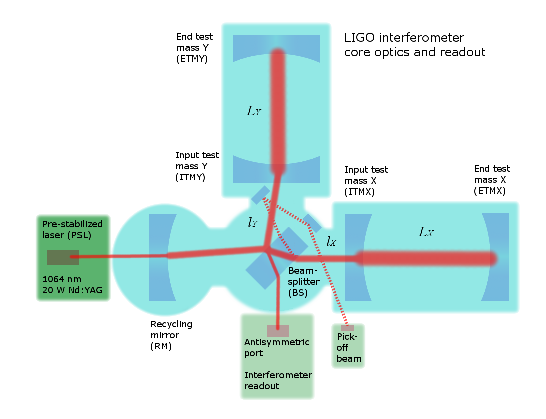
\includegraphics[height=135mm,width=150mm]{figure1.eps}
\caption{Gravitational wave strain $h(t)$ is derived from differential arm motion (DARM), read-out from a photodiode downstream of the antisymmetric port. A small ghost beam from a reflection off an anti-reflective coating, on either the beam-splitter (BS) or an inner test mass (ITM), provides the Michelson (MICH) channel. The DARM readout channel predominantly measures the small change in different arm length, $\delta(L_-) \equiv \delta(L_y - L_x)$, while MICH measures that in the Michelson length $\delta(l_-) \equiv \delta(l_y - l_x)$. There is also a small coupling from $\delta(l_-)$ to the DARM channel. To a lesser extent, changes in the length of PRC, which is defined as $\delta(l_+) \equiv \delta(l_y + l_x)/2$ and is measured in quadrature demodulation with respect to the MICH pick-off, also add noise to DARM.}
\label{arms}
\end{center}
\end{figure}

        %In initial LIGO, for historical interest, but not precisely so in enhanced or advanced LIGO,

        %\begin{eqnarray}
        %\aleph \equiv 4 J_0 (\Gamma) J_1 (\Gamma) P \cos \omega_m t, \label{eq09} \\
        %[L_{-} \rightarrow \textit{AS}_Q] = -\aleph g_{cr}t_sb r_c ' \frac{1}{1 + if/f_c} k \delta L_{-}, \label{eq10} \\
        %[l_{-} \rightarrow \textit{AS}_Q] = \aleph g_{cr} t_{sb} r_c \frac{1}{1+if/f_c} k \delta l_{-}. \label{eq11} \\
        %\end{eqnarray}

        %\begin{figure}[htb]
        %\begin{center]
        %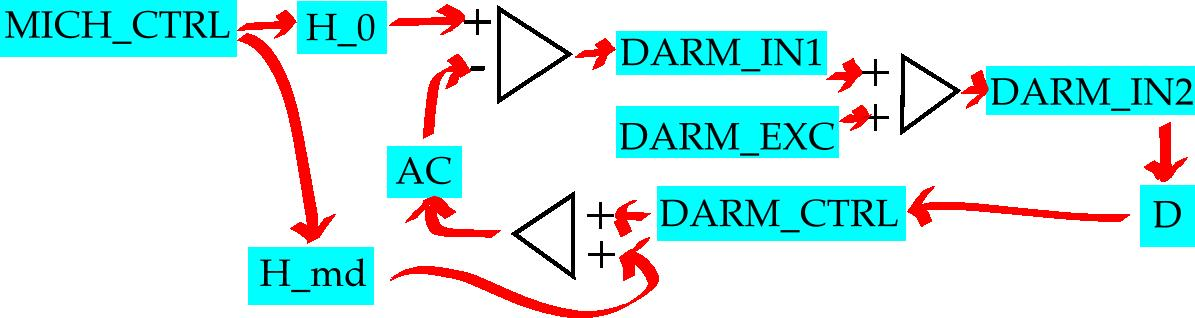
\includegraphics[width = 0.45\paperwidth, keepaspectratio]{servo_loop.jpg}
        %\caption{Servo loop}
        %\label{Servo loop}
        %\end{center}
        %\end{figure}

        The value $\langle L_+\rangle$ is the nominal average arm length, about 4 km in LIGO. The distance function $z(\mathcal{X})$ indicates the distance\footnote{Note that the ITMY distance $z(\textup{ITMY})$ is a function of both the ItMY and BS position}, along the optical path, from the laser to an optic $\mathcal{X}$; the variation $\delta$ denotes a change with respect to nominal value. DARM length is thus defined as $\delta(L_y - L_x)$ and MICH length as $\delta(l_y - l_x)$. In practice, DARM and MICH are the names given to the channels that predominantly measure those quantities. These channels are not so neatly delineated. Unless stated otherwise, the terms DARM, MICH, PRC and CARM will refer to the measured channels, which are related to the lengths through calibration (e.g., DARM = $L_{-} - \pi/(2 \mathcal{F}) l_{-}$ and are cross-contaminated, rather than the physical lengths in Equations~\ref{CARMdef} through~\ref{MICHdef}. 

        As Equation~\ref{DARMdef} and~\ref{MICHdef} imply and Figure~\ref{arms} illustrates, MICH physically ambiguates DARM, which is measured with a photodiode at the interferometer dark port. An arm gain factor $r_{c}'/r_c \approx 139/0.990$, where $r_c$ is the arm cavity reflectivity for the LIGO laser carrier frequency and $r_{c}'$ is the derivative of $r_c$ with respect to round trip phase~\cite{ReadoutGWA,BallmerThesis} (c.f., cavity finesse $\mathcal{F} \approx 219$). This factor amplifies DARM motion for Initial and Enhanced LIGO, given by Equation~\ref{rcfactor}:

        \begin{eqnarray}
        r_{c}' = \frac{2 \mathcal{F}}{\pi} \approx (139/0.990)\times r_c. \label{rcfactor}
        \end{eqnarray}

        \textit{A priori} MICH noise will leak into measurements of DARM with a frequency-independent transfer function equal to the coefficient of Equation~\ref{rcfactor}. Empirically, coherence measurements confirm this coupling is the dominant part of the transfer function, but frequency-dependent residuals suggest other effects exist. PRC is also indirectly correlated with DARM. Independent photodiodes for MICH and PRC, used for feedback, their respective auxiliary length control servos, provide the witness channels for cancelling cross-talk into DARM. These receive a ghost beam from an internal reflection in the beam-splitter. This beam carries a radio-frequency modulation; one demodulation quadrature provides MICH, the other PRC.

        \subsection{Auxiliary noise coherence at sensitive frequencies}
        \label{aux_noise}

	 Cross-talk can be quantified with coherence, the Fourier frequency-dependent analog of statistical correlation. On a scale of 0 (none) to 1 (full), coherence represents the normalized fraction of power of a frequency bin in the spectrum of one channel that can be found in the same frequency bin in the spectrum of another channel. The coherence at a given frequency $f$ and time $t$~\cite{Boashash1990} is given by Equation~\ref{coherenceDef}, where $P_{xy}$ is cross-power spectral density as in Equation~\ref{Pyx}. False alarm rate for a coherence measure is governed by the probability that an observed coherence $C_{\textup{obs}}$ is greater than the actual coherence $C$. For a window factor $w$ (0.95 for a Hann window) and $N$ sample averages is described, for Gaussian noise, in~\cite{MendellCohere2013} by Equation~\ref{CohereProb}
\begin{eqnarray}
C_{xy}(f, t) = \sqrt{\frac{\left| P_{xy}(f, t) \right|^2}{P_{xx}(f, t) P_{yy} (f, t)}}\label{coherenceDef}, \\
Prob\left( C_{\textup{obs}}^2 > C^2\right) = \left(1-C^2\right)^{w(N-1)} \label{CohereProb}
\end{eqnarray}

Uncorrelated channels have low coherence. Strain, $h(t)$, is measurably coherent with MICH and PRC, as seen in Figure~\ref{coherenceGraph}. MICH-DARM coherence, hence noise coupling, is sometimes as large as 0.1 in the 100 to 300 Hz band for the LIGO Hanford Observatory detector H1. Problematically, this is the most sensitive band for Initial and Enhanced LIGO. 


	Allen, Hua, and Ottewill~\cite{AllenHuaOttewill1999} first posited the filtering scheme that this paper employs. Where there is a strong correlation between a signal channel and a noise channel, the noise can be partially cancelled if a noise-to-signal transfer function, convolved with noise, is applied to the measured signal. Auxiliary MICH-PRC Subtraction (AMPS), a Matlab~\cite{Matlab2012a} pipeline, realizes this procedure.

AMPS fits a filter onto the most coherent frequency band of the noise-to-signal transfer function. It processes LIGO Science Run 6 segment-by-segment, subdiving each segment into windows up to 1024 seconds in duration. S6 LIGO science segments exhibit MICH and PRC cross-talk primarily from 50 to 400 Hz. DARM is calibrated through a linear, frequency-dependent filter~\cite{LIGOCal2010} into the scientific channel Hoft, corresponding to observed $h(t)$ in units of strain. Since coherence and the technique of Allen, Hua, and Ottewill are both linear and transitive, AMPS has been designed to analyze Hoft data rather than analyzing DARM and duplicating the calibration filter.

Transfer function fitting is weighted toward 50-400 Hz by design in AMPS. Each transfer function for a given 1024 s of data is the average of 1024 independent ratios-of-FFTs (2047 Hann-windowed, 50\%-overlapping FFTs of 1 s samples of the 1024 s). Since the error in an FFT scales with the inverse square root of the number of averages, the relative accuracy for the transfer function is $\mathcal{O}\left(1024^{-1/2}\right)$. AMPS can proceed with less data, as little as 32 s, which yield $\mathcal{O}\left(32^{-1/2}\right)$ relative accuracy. Outside the 50-400 Hz band, the program deweights the fit to the transfer function and pre-processes it, suppressing it by factors of $(f/f_\textup{knee})^\alpha$, where $\alpha = 8$ at low frequencies and $-8$ at high, where $f_\textup{knee}$ was respectively 50 and 400 Hz. AMPS smooths and deweights (Figure~\ref{tfGraph}) known spectral peaks, including 60 Hz harmonics, the LIGO suspension violin modes, and calibration lines. Deweighting and pre-processsing, when carefully tuned, prevent AMPS from confusing the filter design with statistically insignificant transfer function data, which could introduce noise, as well as supporting faster and more accurate fit convergence with fewer free parameters.

% As referenced by Greg Mendell (cite his 2013 March LVC talk if necessary), the statistical significance of a transfer function -- and thus our measure of the coupling from noise into signal -- is assessed through coherence. By fitting only in regions where the coherence was typically greater than 0.03 (CHECK: is this about the right number?), we verified that the uncertainty in our transfer function was no greater than (CHECK: what is the number?). 

 

%avoid monopolizing a scarce set of free parameters, the poles and zeros that float to fit the transfer function.

%By minimizing the transfer function and thus our fitted filter where it would be incoherent, we avoid adding noise.

%        \subsection{Predicted and empirical correction}
%        \label{correction}
%
%            Manual, constant correction long applied, known \textit{a priori} cause.
%
%            Draw on Stefan Ballmer/Rana Adhikari and trace down the origin of the MICH and PRC estimates, possibly reiterate with citation. Emphasize that it is frequency-independent, flat, whereas the observed residual coherence is not perfectly flat.
%
%        \subsection{Filter mathematics: in-loop and out-of-loop}
%        \label{filter_math}
%
%            Mathematics of in-loop/out-of-loop filtering.
%
%            Discuss servos, including the usual terminology of plants, gain. Principle references: Saulson~\cite{Saulson}, Luca Matone's lectures, possibily some EE texts such as Horowitz and Hill.
%
%	We should also quote Jeff Kissel's thesis~\cite{KisselThesis}, which in chapter 3 has an extensive discussion of DARM, its calibration and response function, the actuation and sensing functions, filters and plants.
%
        \subsection{Estimating optimal filters}
        \label{filter_est}

	Parameters for the transfer function are determined by Vectfit, developed by Gustavsen et al.~\cite{Deschrijver2008,Gustavsen2006,Gustavsen1999}. Vectfit iteratively approaches the transfer function. AMPS applies Vectfit to one channel at a time, as will be discussed in Section~\ref{out-of-loop}. Each iteration of Vectfit uses pole-shifting to optimize a rational transfer function model according to a least-squares fit. Empirically, convergence on a model was achieved after about five iterations on S6 data; AMPS chose fifteen iterations for a safety margin. After sufficient iterations, the transfer function model (for AMPS, 32nd order) is extracted. Zero-pole-gain (ZPK) format is used to trim out-of-band zeroes and poles and multiply by a 2nd order Butterworth low-pass filter just below the Nyquist frequency of 8192 Hz, placing poles at 7 kHz to ensure causality. An overall scale factor is applied to the low-pass to keep the filter gain at 150 Hz the same value as the regression in Vectfit. AMPS converts the ZPK model to second-order-section (SOS) digital filter format for numerical stability. Effecting the inverse Fourier transform of Equation~\ref{gcf}, the SOS filter is then arranged in time-domain format. Finally, the SOS filter is applied to its respective noise channel. The estimated true Hoft signal equals the original Hoft measurement minus the convolution of each filter to its respective noise channel. 

This procedure makes two assumptions. It assumes that the dominant coupling from each noise channel into Hoft is linear. Further, it assumes that 2nd order coupling, from one noise channel into the other and subsequently into Hoft, is negligible. Preliminary results suggest these assumptions are justified approximations.  

	Equations~\ref{Txy} through~\ref{hatsf} capture this method. It is analogous to frequency-domain Gram-Schmidt orthogonalization. Allen, Hua, and Ottewill established the mathematical theory, using superscript $^{(b)}$ to indicate a frequency band that we donate as domain $(f)$. Their Equations~7, 8, and 11 correspond, respectively, to Equations~\ref{Pyx},~\ref{hatsf} and~\ref{Txy} here.

%Reference Allen and Ottewill equations 7, 8, 11, 25
%Note that MICH and PRC are not correlated, so we can approximate the subtraction as diagonal in their many-N case
%Also, estimate the risk of 1-1/F Gaussian non-significant subtraction. Note that we do vetoes!

Transfer function $T$ expressed as cross-power ratio of arbitrary channels $x$ and $y$:

            \begin{eqnarray}
            T_{xy} (f) = \frac{P_{yx}(f)}{P_{xx}(f)}. \label{Txy}
            \end{eqnarray}

\noindent Continuous and discrete definitions of cross-power $P$; the operator $E$ denotes an expectation value, and $p$ and $q$ are discrete indices:
 
            \begin{eqnarray}
            P_{yx} (f) = \int_{-\infty}^{+\infty} \left(\int_{-\infty}^{+\infty} y^{*} (\tau) x(t+\tau) d \tau \right) e^{i 2 \pi f t} dt; \label{Pyx} \\
            P_{yx} (f, t) = \Sigma_{q=-t}^{t} R_{yx} (q) e^{-2 \pi i f q}, \label{Pyxext} \\
            R_{yx} (q) = E\left[ y_{p+q} x_p^* \right] \label{crossCovar}.
            \end{eqnarray}

\noindent Estimated feedforward filter $g$ as an inverse Fourier transform $\mathcal{F}^{-1}$, decoupling signal (subscript $s$) from noise (subscript $n$):
            \begin{eqnarray}
            g(t) = \mathcal{F}^{-1} \left( \textup{fit} \left[ T_{sn} (f) \right] \right) \label{gcf}.
            \end{eqnarray}
\noindent Post-filtering signal $\hat{s}$ in terms of convolution (the $\times$ sign) with $\gamma$, the transfer function coupling noise into signal, $s$ pre-filter signal, $n$ noise, and with channels indexed by $j$ and curly brackets indicating an observable quantity: 
            \begin{eqnarray}
            \hat{s} (t) = \left\{ s + \Sigma_j \left(\gamma_j \times n_j\right)\right\} (t) - \Sigma_j \left(g_{j} (t) \times \left\{ n_{j} \right\} (t)\right) \label{hatsf}.
            \end{eqnarray}

%\noindent where $T$ denotes a transfer function, $P$ a cross-power, $\hat{s}$ is the post-filter signal, $s$ is the pre-filter signal, $n$ is the noise, $g_s$ is the transfer function coupling noise into signal, $g_c$ is the estimated feedforward filter decoupling noise from signal, and the subscript $j$ indexes different channels. Angle brackets indicate an observable or measurable quantity. The operator $E$ denotes an expectation value, and $p$ and $q$ are discrete indices.

Application of this paper's method to uncorrelated channels would lead to unwarranted noise reduction by an analytic factor of $(1 - 1/F)$~\cite{AllenHuaOttewill1999}, where F is the number of bins in a fitted frequency span, or, in time-domain, the number of averages. Given 1-s windowing with 50\%-overlap on 1024 s, $F = 2047$, for an unwarranted noise reduction of about 0.05\%. The ideal of 1024 s windows is not always achievable with LIGO duty cycles. In these cases, AMPS incorporates some filters estimated on as little as 32 s of data, for which the unwarranted reduction would be 3\%, but only when these filters are averaged together with longer-duration (512 s or greater) filters. No isolated filter is estimated on less than 60 s of data, which could yield an uncorrelated noise reduction of 1.5\%. Allen, Hua, and Ottewill clarify that subtraction is tenable so long as covariance (in frequency-domain, coherence) is present at a statistically significant level. They set a benchmark of an order-of-magnitude above the magnitude-square covariance expectation value of $1/F$. Since the AMPS pipeline emphasize fits in regions where the coherence is greater than 3\%, and often 10\% or more, it usually satisfies their criterion.


\begin{figure}
\begin{center}
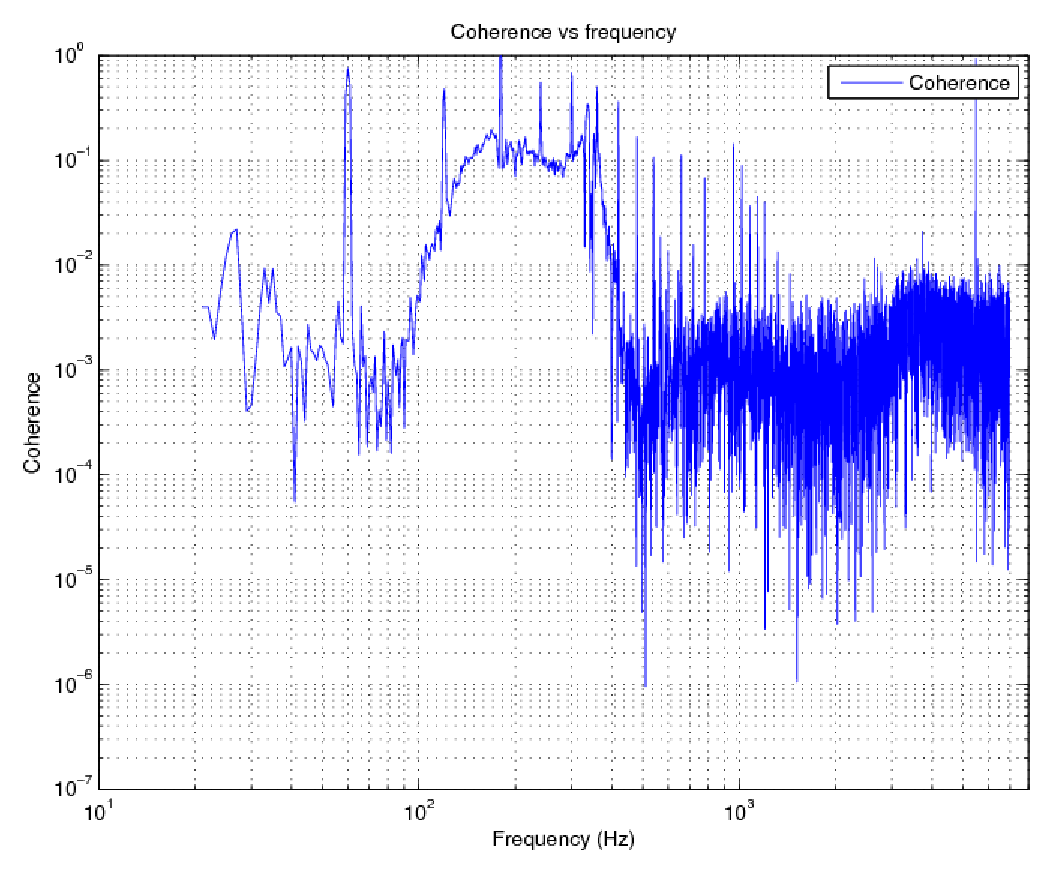
\includegraphics[height=70mm, width=70mm]{figure2a.eps}
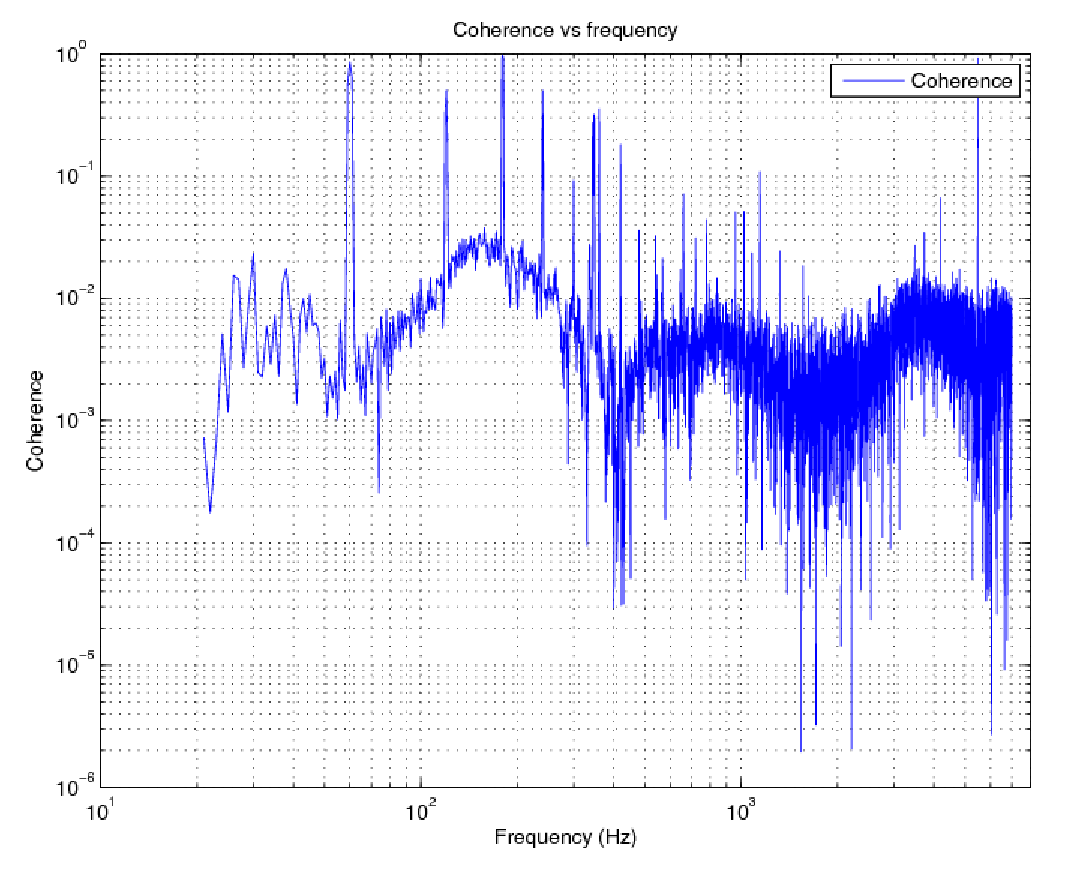
\includegraphics[height=70mm, width=70mm]{figure2b.eps}
\caption{Sample coherence measurements between $h(t)$ and auxiliary control channels for LIGO Hanford Observatory, H1: 2010 March 21. $h(t)$-to-MICH coherence on left, $h(t)$-to-PRC coherence on right. Statistically significant coherence justifies fitting; in frequency bands where coherence rose above background levels, the transfer function fit was weighted more heavily.}
\label{coherenceGraph}
\end{center}
\end{figure}
\begin{figure}
\begin{center}
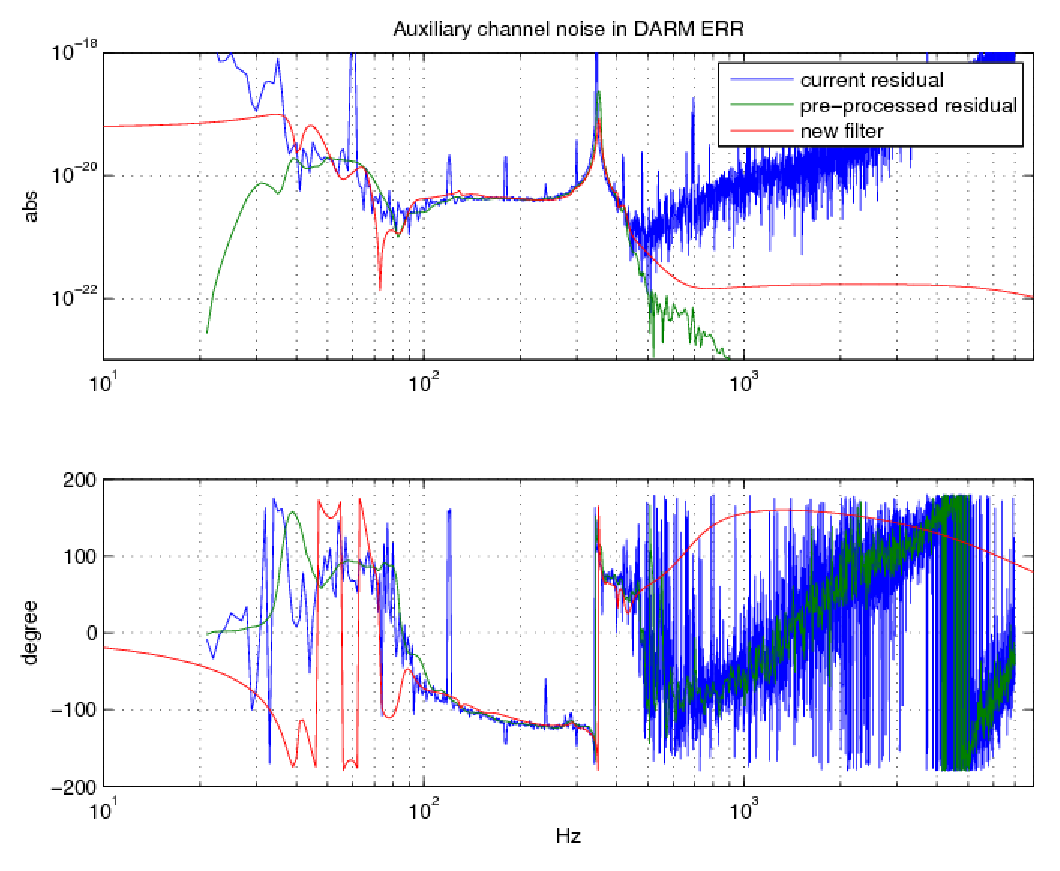
\includegraphics[height=90mm, width=70mm]{figure3a.eps}
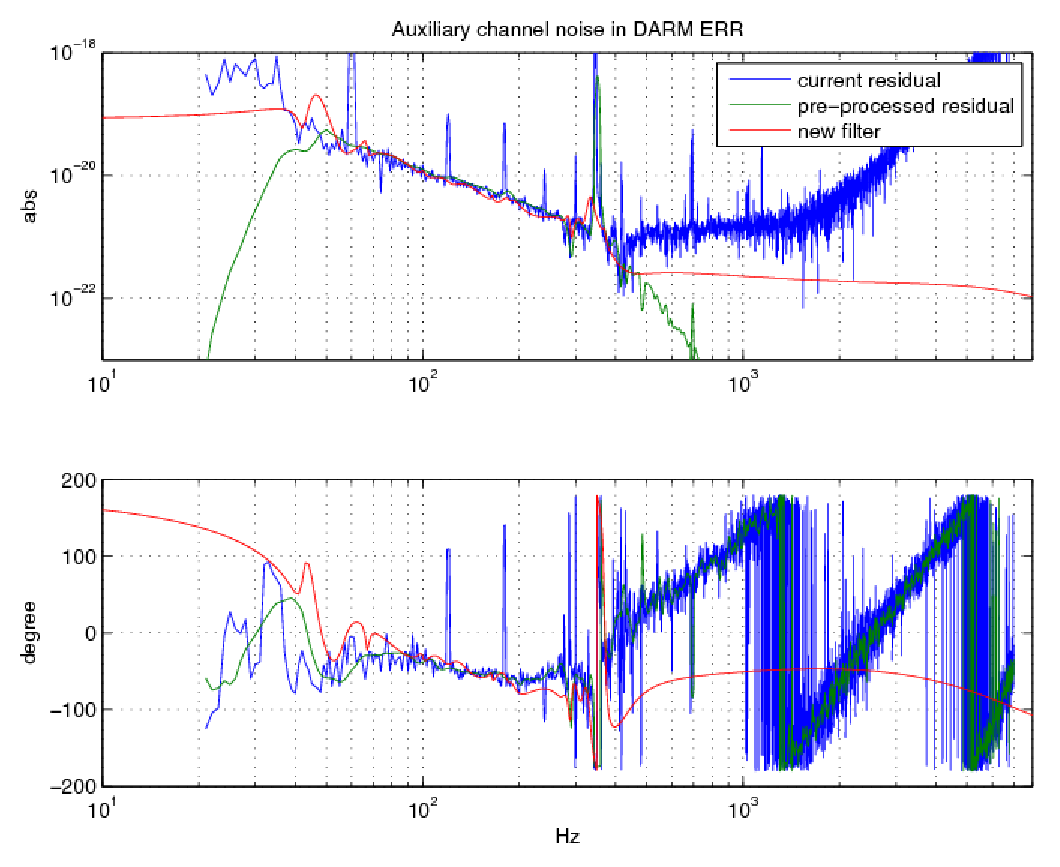
\includegraphics[height=90mm, width=70mm]{figure3b.eps}
\caption{Sample transfer function measurements (amplitude and phase) from LIGO Hanford Observatory, H1: 2010 March 21; MICH on left, PRC on right. Transfer function fit in coherent band -- note the difference between raw data residual and the 'pre-processed residual', which has been smoothed and weighted to emphasize known-coherent bands.}
\label{tfGraph}
\end{center}
\end{figure}
\begin{figure}
\begin{center}
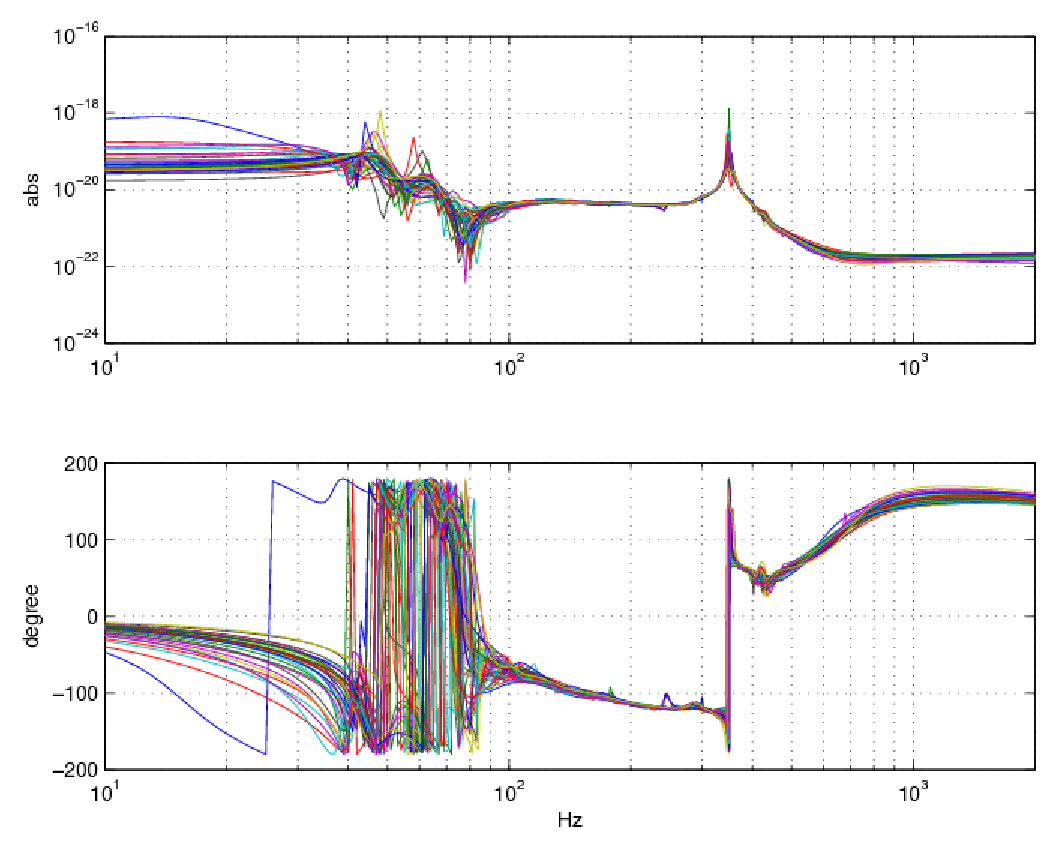
\includegraphics[height=90mm, width=70mm]{figure4a.eps}
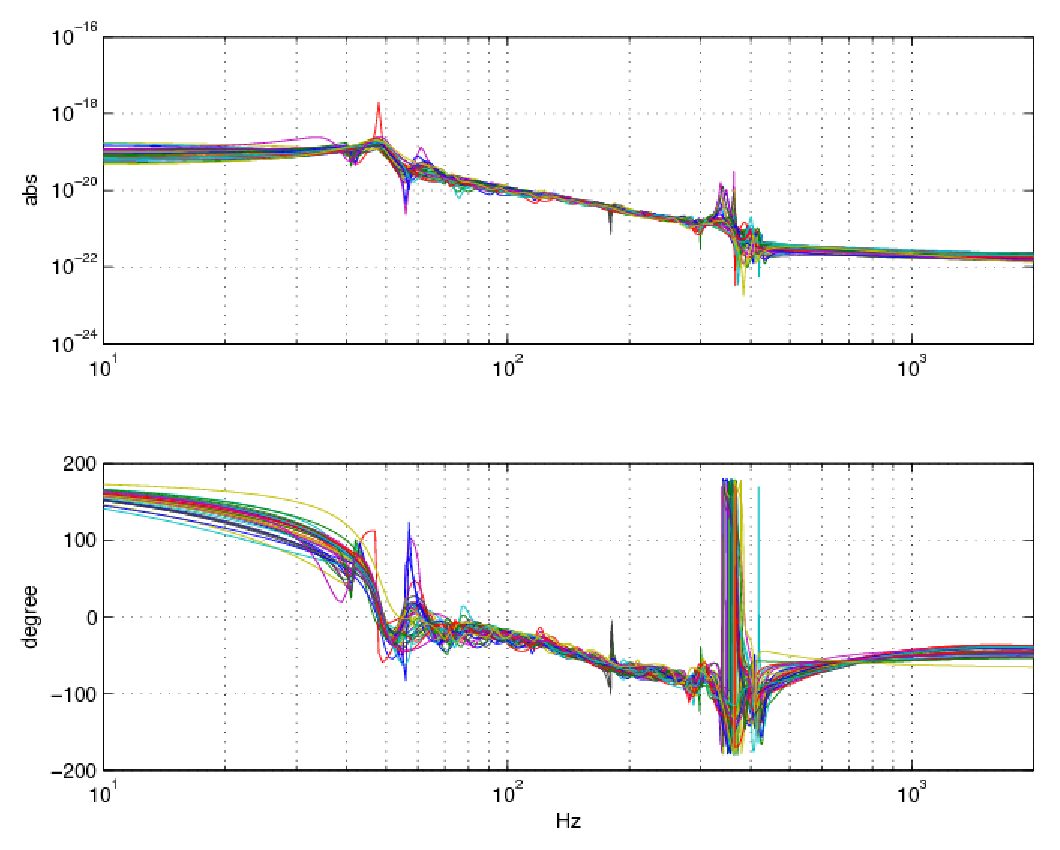
\includegraphics[height=90mm, width=70mm]{figure4b.eps}
\caption{Sample Bode plots of fitted ZPK filter functions (amplitude and phase) for multiple 1024 s windows in a science segment, at LIGO Hanford Observatory, H1: 2010 March 21; MICH on left, PRC on right.}
\label{BodePlots}
\end{center}
\end{figure}
\begin{figure}
\begin{center}
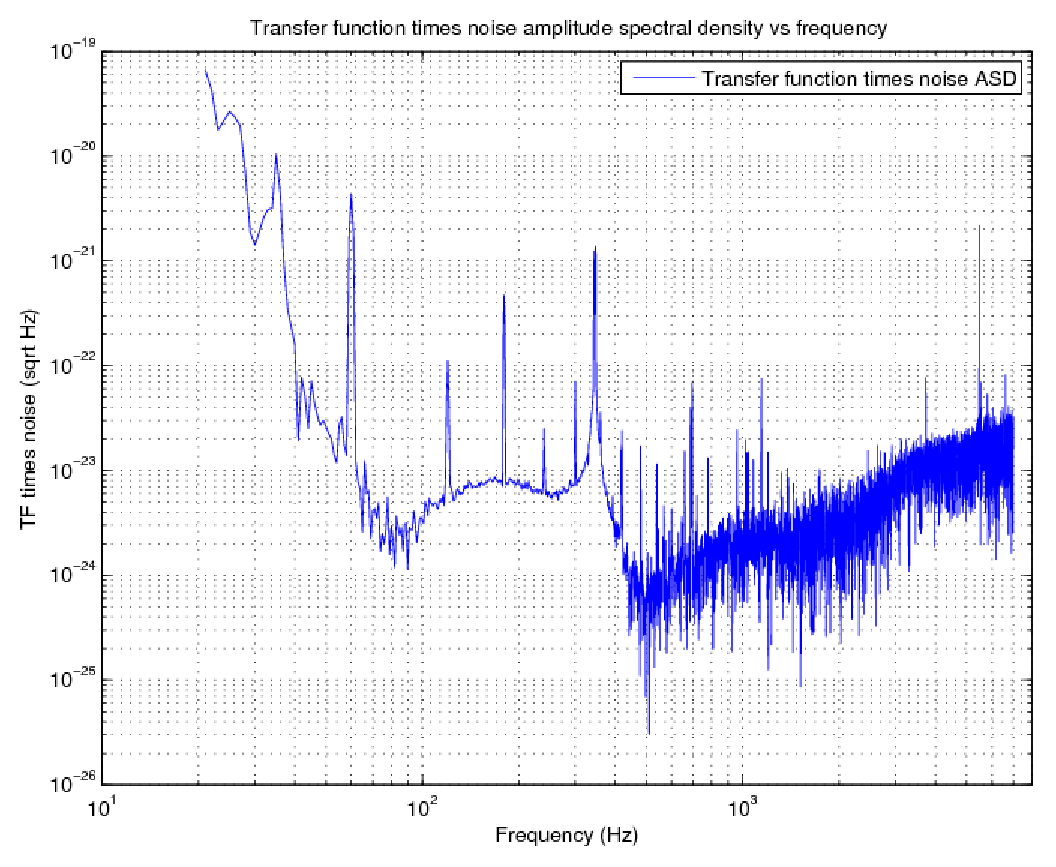
\includegraphics[height=70mm, width=70mm]{figure5a.eps}
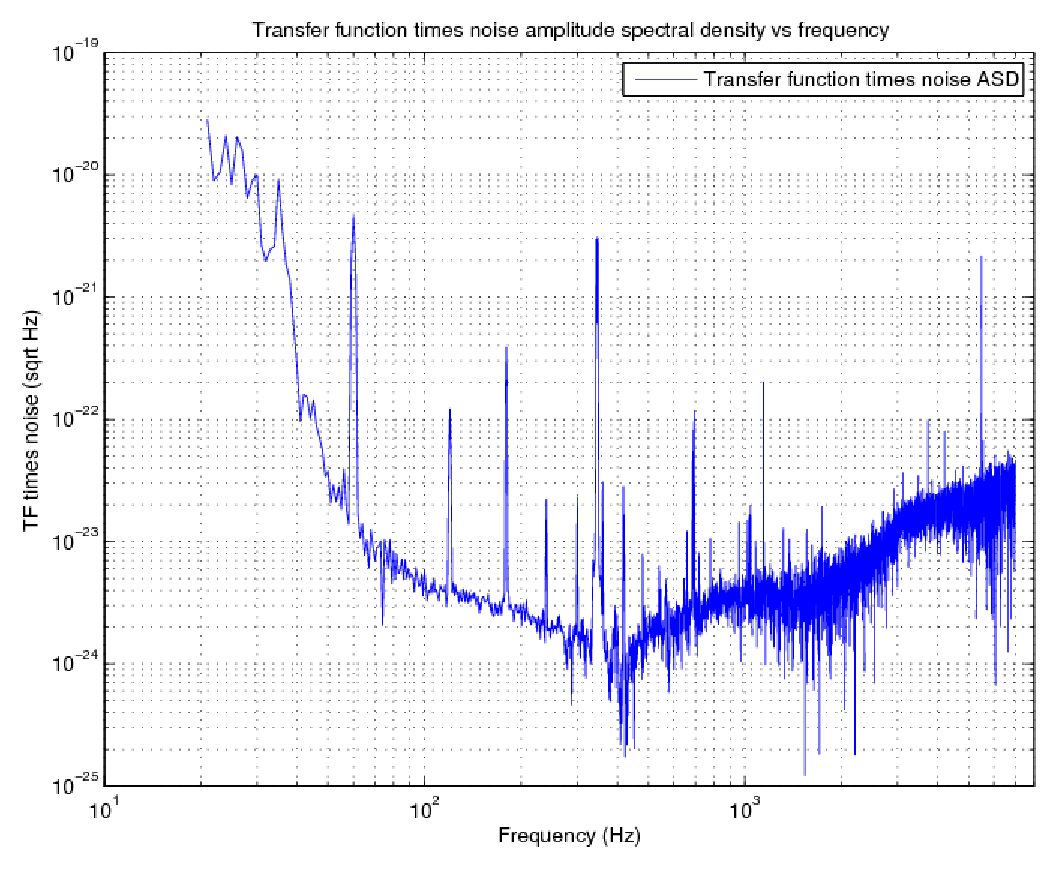
\includegraphics[height=70mm, width=70mm]{figure5b.eps}
\caption{Sample subtracted spectra for one window, representing the applied feedforward corrections for each channel during that window, at LIGO Hanford Observatory, H1: 2010 March 21; MICH on left, PRC on right. }
\label{subtractedSpectrum}
\end{center}
\end{figure}

%We employ Vectfit to design, in Matlab 2012a, a 32nd-order (though the order is flexible) ZPK least-squares fit to the MICH-Hoft and PRC-Hoft transfer functions. The transfer functions are measured over a window up to 1024 s long. We typically take the FFT with 32 averages. The transfer function is weighted and smoothed slightly (Figure 3) to allow the iterative pole-fitting to optimize better. Once the ZPK filter emerges from Vectfit it is converted to second-order sections (SOS) and applied onto the MICH or PRC channel, which is the summed with Hoft, cancelling any leaked noise.

%Our fit heavily weights regions where MICH and PRC are coherent with Hoft (Figure 2), so that we do not fit poles to statistically insignificant frequency bands, as judged by typical coherence values. Thus we avoid introducing excess noise due to inaccurate filter design. To reiterate Section \ref{aux_noise}, the pre-processed TF differs from the raw TF in being deweighted at 60 Hz harmonics, known lines, calibration lines, and the violin modes, and it is reduced by $(f/[50 Hz])^8$ for f < 50 Hz and by $([400 Hz]/f)^8$ for f > 400 Hz. 

As described in Section~\ref{filter_fitting-out-of-loop}, the filters calculated for each 1024-s window are blended to generate the estimated signal for a whole science segment. Figure~\ref{BodePlots} illustrates the short-term consistency of noise transfer functions during a few-hour science segment, presenting a Bode plot of Hoft-MICH transfer function fits for consecutive windows from 2010 March 21 at LIGO Hanford Observatory (magnitude, top and phase, bottom vs frequency [Hz]). These transfer functions varied more markedly over longer timescales of months, reflected in the fluctuating amount of improvement seen in Figures~\ref{typicalInspiralGraph} and~\ref{bestInspiralGraph} (covering $4\times10^6$ seconds of data). Figure~\ref{subtractedSpectrum} presents a sample subtraction for one 1024-s window. These figures show that AMPS successfully, efficiently realizes the intent of Allen, Hua, and Ottewill on operational data for a kilometer-scale gravitational wave interferometer.

Section~\ref{prior_programs} sets this method in context, Section~\ref{safeguards} discusses safeguards and vetos, and Section~\ref{out-of-loop} discusses the details of implementation and verification.


% We will return to the issue of windowing and the tests and safeguards thereby enabled, but first a brief overview of alternatives to Vectfit is in order.

    \section{Feedforward in-loop and alternative programs}
    \label{prior_programs}
   
        During LIGO running, real-time feedforward filtering for MICH and PRC noise must meet operational constraints. Alternative methods, such as the Wiener filtering now being considered for seismic and gravity-gradient cancellation, are possible for this project~\cite{Driggers2012ActiveNoise}. Vectfit and a classical frequency-domain transfer function fit appear most productive for the reasons described below.
        
        \subsection{Manually-designed rational filtering}
        \label{manual_design}

            Manual designs of feedforward functions prove time-consuming. Transfer functions can be approximately fit using the LIGO Foton filtering system~\cite{Sigg2005}. Several additional transfer function measurements are needed for a filter deployed in-loop, in order to compensate for servo loop gain and actuation functions. Manual design is not an efficient alternative to algorithmic transfer function design: it is labor-intensive to repeat regularly, and the results of our run over S6 suggest that filter redesign should be performed often.

        \subsection{Vector-fitted filter functions}
        \label{vectfit}

            Algorithmic fitters such as Vectfit allow adaptive design of transfer functions. Since the dynamic range in magnitude for LIGO length control channels, and consequently transfer functions, can vary over tens of orders of magnitude, one must take care to weight and pre-process data, especially when operating in the most sensitive band from 100 to 300 Hz. Although not the only possibility, Vectfit, applied to a single noise-signal pair, is straightforward. Vectfit iterates a rough \textit{prior} set of pole locations, translating it across the complex plane according to a least-squares fit of the rational function onto transfer function data. About five iterations achieve good convergence. AMPS employs Vectfit's report on cumulative goodness-of-fit, root-mean-square (RMS) error, as a statistic to decide whether to reject Vectfit's filter regression. Using this statistic allows AMPS to isolate a failure in regression to one channel. From empirical studies, RMS error above $1\times 10^{-18}$ indicates a poor fit, where the fit residual of frequency bin $i$ is $\Delta_i$ ($i \in [1,...,N]$), and RMS error $\sigma$ is defined by Equation~\ref{RMSerrorDefinition}:

\begin{eqnarray}
\sigma = \frac{\sqrt{\Sigma_{i=1}^N \left| \Delta_i \right|^2}}{\sqrt{N}}\label{RMSerrorDefinition}.
\end{eqnarray}

        \subsection{Wiener filters}
        \label{wiener_filters}

            Wiener filtering~\cite{Wiener1949} searches for an optimal filter of a particular kind: it minimizes the squared error of the residual. That error can be the difference between the estimated signal and the time-delayed signal. However, the error is over the entire spectrum. Data over the dynamic range of LIGO's bucket appears to call for band-passing the spectrum into sub-spectra. Evaluating the error over sub-spectra could circumvent contamination from the high spectral power present at low-frequencies. Coherence at low-frequencies is low, but a Wiener filter by default will fit their high-power at the expense of lower-power, higher frequency bands. That fit would be statistical unsubstantiated and counterproductive, if calculated for the entire spectrum at once. Transforms that break the spectrum up into many bands, such as wavelet transforms~\cite{KlimenkoSite}, seem promising. Filters that intentionally focus on bands with high RMS power, such as seismic and gravity gradient noise, can use Wiener filtering without difficulties. At the Caltech 40m, Wiener filtering has solved many issues with Newtonian and seismic noise~\cite{Driggers2012ActiveNoise}.

%    \section{Feedforward in-loop}
%    \label{in-loop}

        %\subsection{Filter fitting in-loop}
        %\label{filter_fitting_in-loop}

        %    In loop, in real-time, feedforward filtering can prove even more 

        \subsection{Real-time in-loop filtering}
        \label{real-time}
      
            Auxiliary MICH-PRC Subtraction (AMPS) code, as presented by this paper, is designed to provide out-of-loop, post-facto Vectfit feedforward filtering that meets criteria for statistically soundness and accuracy. The software must also be efficient. Auxiliary MICH-PRC Subtraction code runs a few times faster than real-time on 2013 hardware whilst conducting extensive tests and safeguards, documented in Section~\ref{safeguards}. Subsequent versions might be considered for use in real-time. Unfortunately, failing the veto triggers extends the time-to-completion. Long program time is acceptable for a side-channel generating in data when a reference $h(t)$ already exists. This arrangement is not ideal for in-loop, real-time production of $h(t)$. Even if the vetos are not triggered, the maximum time delay between an $h(t)$ sample and its final, corrected form is the time at which the filter is generated, up to a window (1024-s) in the future. This lag is undesirable for electromagnetic follow-up, part of the multi-messenger astronomy~\cite{Swift2012,Antares2013} desired for Advanced LIGO. A modified system that could operate in real-time, refreshing periodically with prior data from the same science segment, might be useful for countering upconversion and other non-linear features of cross-coupling.

\section{Safeguards and vetoes}
\label{safeguards}

    \subsection{Runtime safeguards}
    \label{runtimeSafeguards}

Gravitational wave strain, $h(t)$, is the most important data channel for LIGO; the AMPS pipeline takes several measures to ensure its integrity. Post-facto adjustments are unusual; when individual LIGO searches process $h(t)$, they typically do not apply any correction based on auxiliary channel data. Such corrections have been the province of real-time servos. Given the new approach here, AMPS verifies data integrity through several safeguards and vetoes against known and possible issues. These issues include making data worse, offsetting and incorrectly time-stamping the data, incorrectly subtracting $h(t)$ from itself, and introducing Fourier transform windowing artifacts.

After filtering each window, AMPS calculates its amplitude spectral density in Matlab using pwelch~\cite{Matlab2012a,Welch1967}, which enables calculating inspiral range $\mathcal{R}$, an astrophysical measure of performance~\cite{FinnInspiral1993} and quantifying  the change in spectrum. The window's filtered data is used, if post-filter $\mathcal{R}$ is at least 99.9\% of unfiltered $\mathcal{R}$, and if none of the 40 points in a `comb' (each point being 5/16 Hz wide) of quiet bands is noisier in $h(t)$ than 1.2 times $h(t)$ in unfiltered data. If the window fails this test, it is passed back through the windowing method and combined with baseline, unfiltered LIGO data from the same window until it passed the veto. This process allows for progressive diminuation of the influence of any abrupt non-stationary features in the transfer function that may be causing the test to fail. After eight such `re-normalizing' cycles are made -- failing which, it then writes what it has and proceeds to the next segment. Empirically, it is found that these criteria ensure that almost all AMPS data is better, on average, than Hoft raw data (HOFT in Figure~\ref{pipelineGraph}), because it selects the better of either baseline or filtered $h(t)$.

    \subsection{Post-processing safeguards}
    \label{postprocessingSafeguards}

Besides imposing these runtime safeguards, the AMPS project computes diagnostics to check whether calibration lines (Figure~\ref{calLineTest}) are diminished -- which would indicate that AMPS was incorrectly subtracting $h(t)$ signal from the HOFT channel. It also checks whether injections (Figures~\ref{timeDomainInjection} and \ref{crossCorrelationGraph}) are recovered at the correct times. These injection studies examine compact binary coalescence and sine-Gaussian hardware injections~\cite{LIGOBurst2012} for GPS seconds $931.0 \times 10^6$ (2009 July 07) to $932.8 \times 10^6$ (2009 July 28) and produced basic time-domain plots and cross-correlations. In addition, to verify that the ability to observe compact binary coalescences is not decreased by AMPS, we calculate the matched-filter signal-to-noise ratio of each of the compact binary coalescence hardware injections in the S6 data. This is done by filtering each hardware injection against the compact binary coalescence waveform that was used when the hardware injection was performed. The matched filter signal-to-noise ratio is directly proportional to the distance at which such a signal can be observed, and therefore also to the overall sensitivity of the instrument to signals of that type~\cite{Findchirp2012,PetersMatthews1963}. These tests affirmed the result that feedforward data contains recoverable (and slightly higher signal-to-noise ratio) injections.

Calibration line studies seek to answer two questions: whether feedforward distorts the signal and whether it adds noise. The latter question is answered in the affirmative if we find windowing artifacts, such as spectral combs with spacing of 1/1024 or 1/512 Hz, that might be generated around a prominent line. Post-processing tools saw no new combs in our 1800-s, 50\%-overlapping Hann-windowed SFTs before/after comparison of  approximately $10^6$ s of H1 science time between GPS times $931.0 \times 10^6$ (2009 July 07) and $932.8 \times 10^6$ (2009 July 28). The 393.1 Hz calibration line\footnote{Strictly speaking, the line visible in $h(t)$ is a residual artifact from the imperfect cancellation of control and error signals used in the construction of $h(t)$ from the DARM error and DARM control signals. The accidental nature of the line does not affect our analysis, because neither MICH nor PRC affect the line.} exhibited no noticeable comb artifacts. The signal-distortion question is answered by taking the mean of the three 1/1800 bins in the range of [393.1 - 1/1800, 393.1 + 1/1800] Hz: for the $10^6$ s of H1 science time analyzed, the before-feedforward mean was $1.3082 \times 10^{-21} (\textup{Hz})^{-1/2}$, whereas afterward it was $1.3128 \times 10^{-21} (\textup{Hz})^{-1/2}$. Feedforward made the calibration line region noisier by $4.6 \times 10^{-24} (\textup{Hz})^{-1/2}$ or 0.35\%. Evaluating the three bins around the calibration line helps to account for possible spectral leakage, since the central line is much larger than its neighbors. 

%[IN PROGRESS: a quick look at the 2013-06-05 spec avg files shows the five bins centered around 393.10 Hz, with bin width 1/1800 Hz, were, for harmonic mean: before feedforward (2.48308e-23, 4.00795e-22, 8.01098e-22, 4.01188e-22, 2.45973e-23), after feedforward (2.50184e-23, 4.02222e-22, 8.03892e-22, 4.02636e-22, 2.47577e-23) -- this looks within statistical fluctuations, and I think we're safe]. 

We conclude that we are not subtracting Hoft/DARM from itself. The additional noise is perhaps due to the low weighting of the AMPS transfer function fit at the 393.1 Hz line: that part of the spectrum is not tightly fit, because it could bias more sensitive parts of the spectrum.

\begin{figure}
\begin{center}
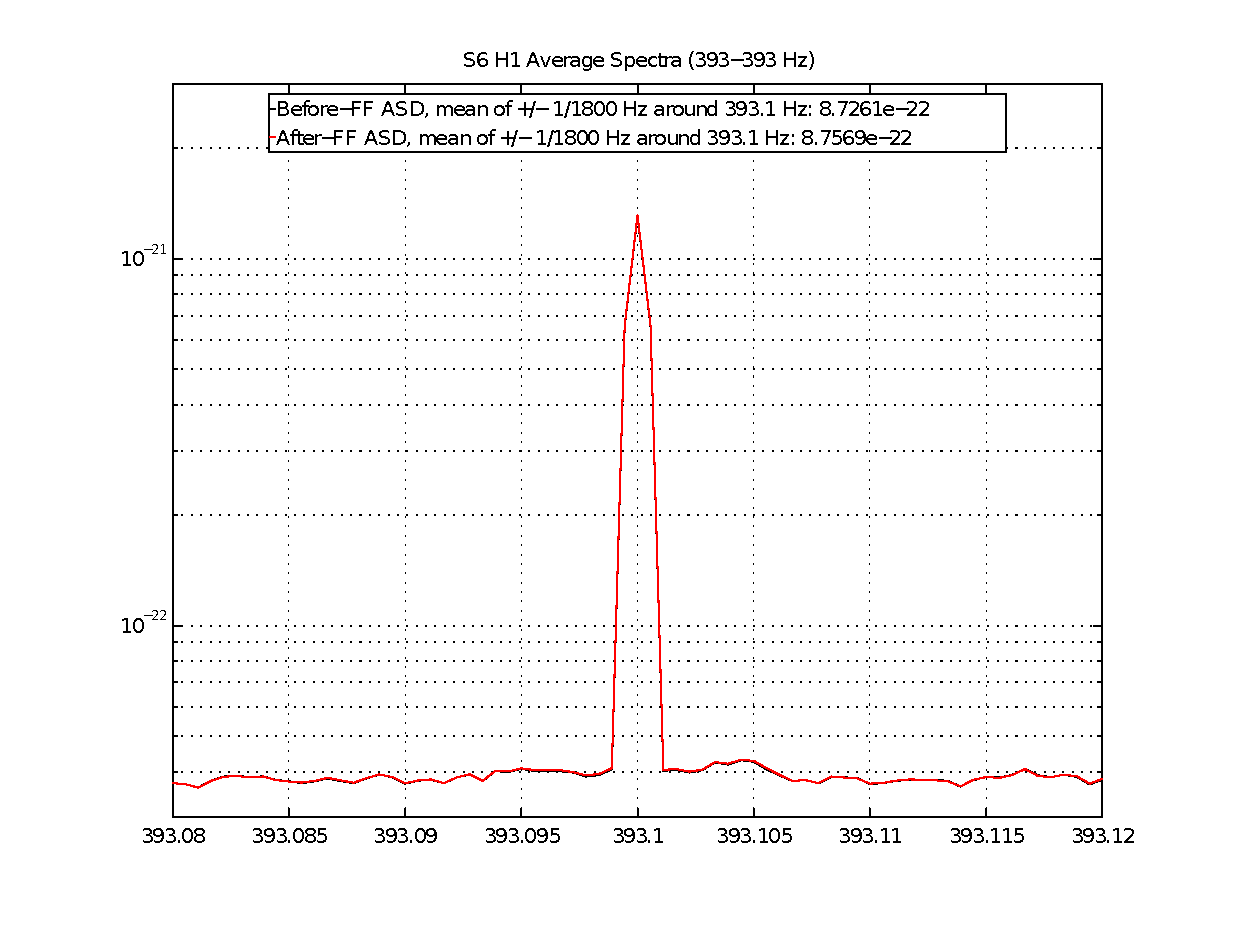
\includegraphics[height=75mm, width=150mm]{figure6.eps}
\caption{Calibration line test: before-feedforward mean of the 393.1 Hz line and two neighboring FFT bins was $1.3082 \times 10^{-21}$, after was $1.3128 \times 10^{-21}$. Feedforward made the calibration line region noisier by $4.6 \times 10^{-24}$ or 0.35\%, suggesting that we correctly apply Hann-windowed feedforward without subtracting true $h(t)$ signal. Moreover, no spectral line combs are observed to either side of the calibration line peak at 393.1 Hz, indicating that the method does not introduce windowing artifacts.}
\label{calLineTest}
\end{center}
\end{figure}

\begin{figure}
\begin{center}
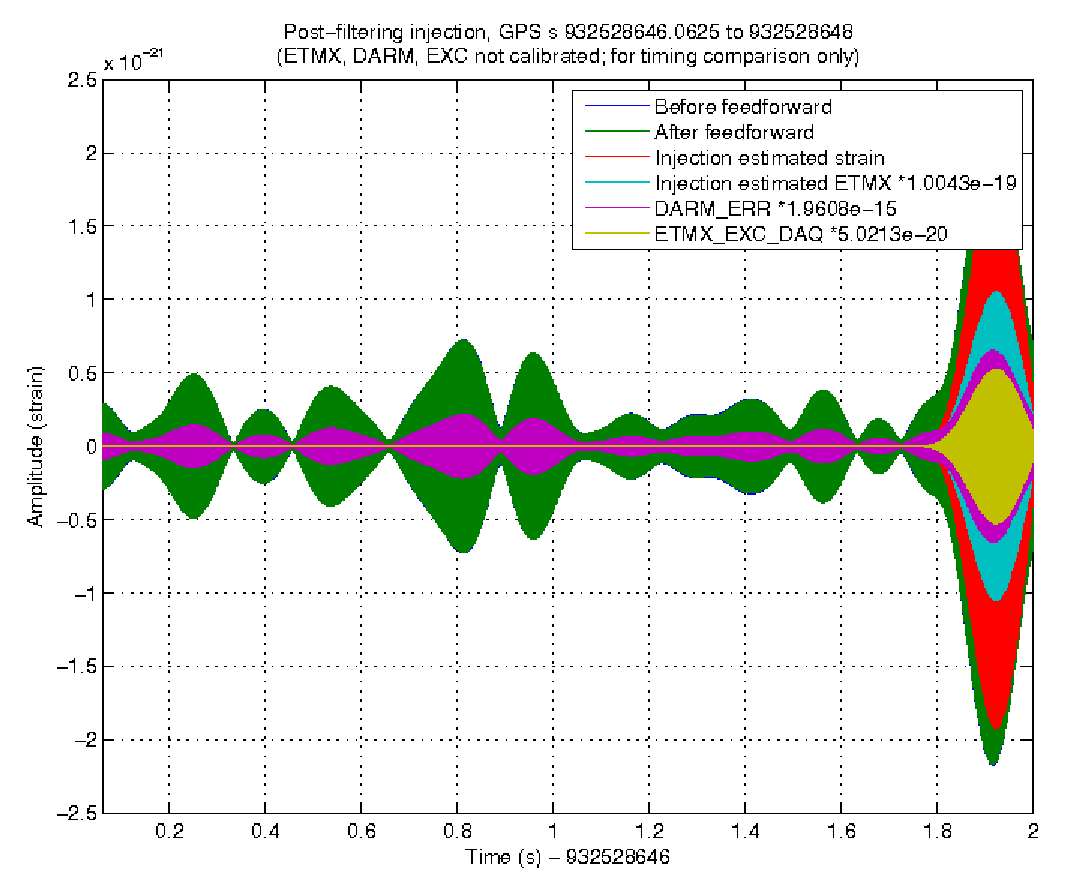
\includegraphics[height=75mm, width=150mm]{figure7.eps}
\caption{Time-domain plot of diagnostic channels from a burst injection: the simultaneous envelope increase after 1.8 s indicates that the burst injection is correctly time-stamped in the new data. Before-feedforward and after-feedforward traces occult each other in the graph, because they are almost identical.}
\label{timeDomainInjection}
\end{center}
\end{figure}

\begin{figure}
\begin{center}
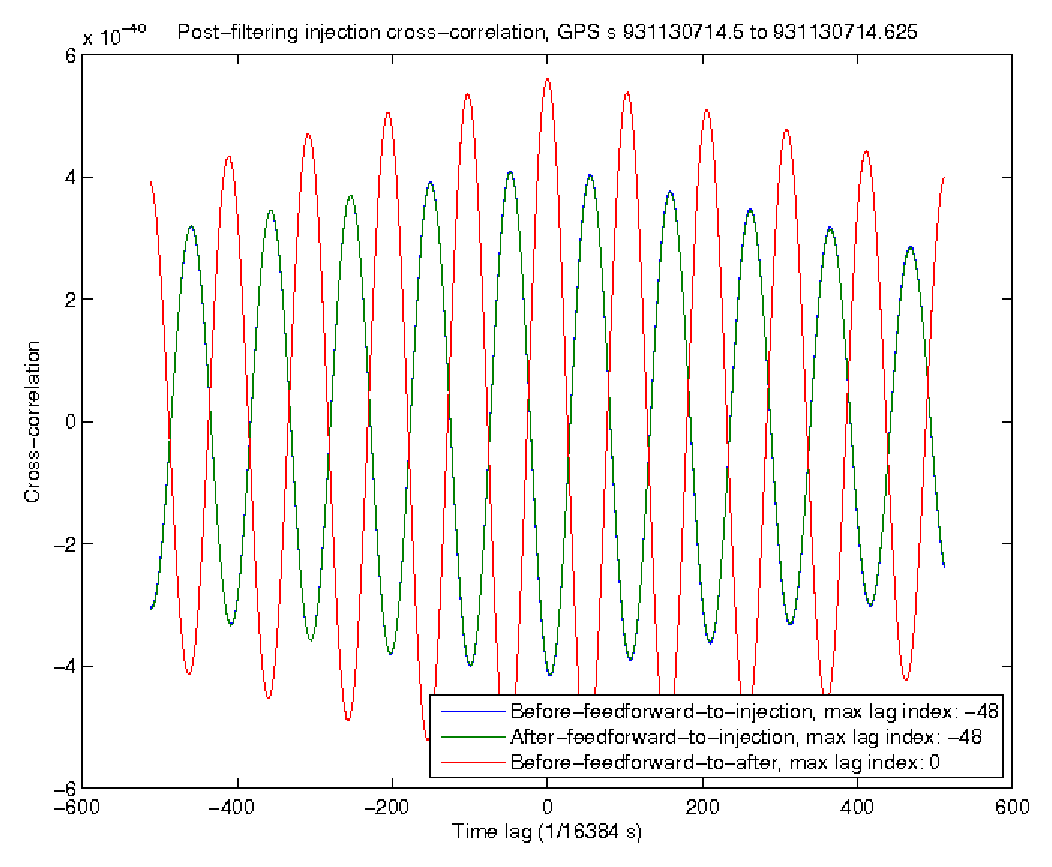
\includegraphics[height=75mm, width=150mm]{figure8.eps}
\caption{Cross-correlation pairwise between pre-, post-feedforward, and injection data: the extrema and zero-crossings match.  Note both before-feedforward (blue) and after-feedforward (green) strain traces are almost identical and therefore overlap. The strains appear inverted, but in the same way, due to a sign error in the hardware injections at this time.}
\label{crossCorrelationGraph}
\end{center}
\end{figure}

        From the nearly equal height of the calibration line before and after and the identical lag of the before and after feedforward strains with respect to the injection, we have confidence that AMPS is not subtracting true $h(t)$ signal from itself, and that it is not shifting the samples in time.

    \section{Feedforward applied to MICH and PRC channels}
    \label{out-of-loop}

\begin{figure}
\begin{center}
%\includegraphics[height=110mm,bb=25 169 579 609]{jm.fig5.eps}
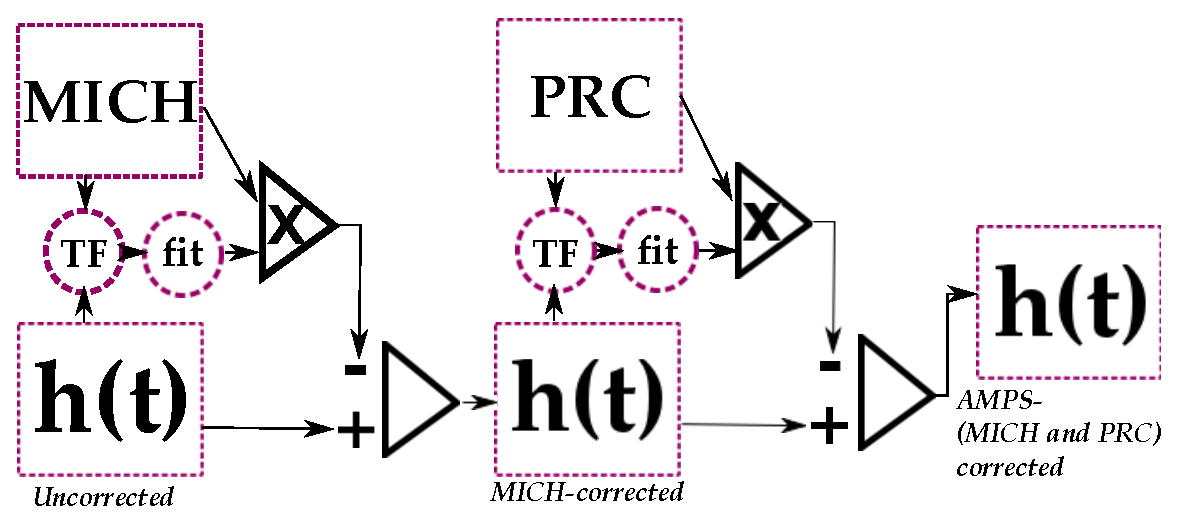
\includegraphics[height=85mm,width=120mm]{figure9.eps}
\caption{Feedforward filtering pipeline to read in Hoft (calibrated DARM), MICH, PRC, and write out AMPS (clean calibrated DARM). Code can be found in the LIGO Matapps SVN: \texttt{matapps/packages/detchar/AMPS/trunk/aletheia.m}}
\label{pipelineGraph}
\end{center}
\end{figure}    
%\textup{Read in Hoft (calibrated DARM), MICH, PRC, write out AMPS (clean calibrated DARM). Code in LIGO SVN:}\\
%\texttt{matapps/packages/detchar/} \\ 
%\texttt{AMPS/trunk/aletheia.m}
%\\

Realizing a post-facto, linear filtering engine, AMPS includes \texttt{aletheia.m}, a Matlab function in the Auxiliary MICH-PRC Subtraction package that fits and applies a filter to either MICH or PRC (specified by an argument). The fit occurs in the frequency-domain. The filter is applied in the time domain. From a high-level perspective, it is a system for reading in Hoft frames, correcting them with MICH and PRC frames, and writing AMPS data frames, accompanied by data quality and state vector channels, and producing diagnostic graphs. The pipeline is shown in Figure~\ref{pipelineGraph}. 

%        A critical point: we use the entire set of data for a window to produce a filter, then apply that filter back to the entire set of data. Those familiar with a machine learning view may worry that this is overfitting, that we are not training the data. But that worry really is not justified. The concept of training and over-fitting are valid in the frequency-domain aspect of this work, where we take steps to correct it, such as the pre-processing of the spectrum shape and the post-processing vetos. But in the time-domain, overfit should we restrict the filter-training to a subset of the data? That might make sense if we assumed the data to be stationary and were going to let it run into the future, or if we wanted to learn something scientific about the meaing of the filter coefficients. None of those assumptions hold. We assume the data to be non-stationary, although a complaint could be made that we are unsure about the timescales of non-stationarity. We do not let the filter run arbitrarily into the future, but explicitly window it. Finally, we do not have ambitions to extract scientific meaning from the filter coefficients, although that may change -- even if we did go down that route, it would probably be based more on the original spectra than on the fit to them.

        \subsection{Filter fitting across science segments}
        \label{filter_fitting-out-of-loop}

So as to run efficiently on a LIGO computing cluster, the AMPS pipeline processes one filtering job per science segment. LIGO science segments range in duration from seconds to days, with the median segment typically lasting hours. During each segment, the interferometer is continuously locked, meaning it is held fixed on one interferometric fringe, by servo controlling all degrees of freedom so that they are stationary. If lock is lost, the segment ends. Serious noise degradations of the signal can also define the end of a segment. Each segment is managed by the main AMPS program, \texttt{eleutheria.m}. This program windows the segment, with windows up to 1024 s long, passes them to the filtering function and merges them smoothly together using 50\%-overlapping Hann windowing. Windowing is idempotent for HOFT; the only difference from window to window is the correction signal added to HOFT. The first 512 s are entirely driven by the first window; every 512 s thereafter, a new window is introduced, as in Figure~\ref{windowingScience}: 

            Because of computing cluster constraints on job time, AMPS breaks up long science segments so that no job processes more than 16384 s of data; these subdivided science segments overlap slightly so that each side would calculate identical filters for the overlap(s), but only the latter half writes the frames for the overlap, avoiding race conditions. Moreover, AMPS does not process science segments shorter than 60 s in the segment list, and science segments with dangling windows shorter than 32 s (after segment subdivision) have those windows rolled into their predecessors so as not to generate a filter based on insufficient data. Finally, AMPS implements range and comb tests to veto filtered windows if they look worse than unfiltered data, as discussed in Section~\ref{safeguards}. 

\begin{figure}
\begin{center}
\includegraphics[height=110mm,width=150mm]{figure10.eps}
\caption{A depiction of windowing for one cluster job, containing one LIGO science segment, illustrates windowing after an initial half-window offset. Filters are calculated for 1024-s windows, then the 50\%-overlapping Hann windows merged, whereupon AMPS $h(t)$ frames are written. Code can be found in the LIGO Matapps SVN: \texttt{matapps/packages/detchar/AMPS/trunk/eleutheria.m}}
\label{windowingScience}
\end{center}
\end{figure}
%One job per science segment, filters are calculated for 1024 s windows; 50\%-overlapping Hann windows merged, AMPS h(t) frames written. Code in LIGO SVN:\\
%\texttt{matapps/packages/detchar/}\\
%\texttt{AMPS/trunk/eleutheria.m}

        %\subsection{Data frame generation}
        %\label{data_frames}
        %
        %    Matlab: write frame files on cluster.

        \subsection{Post-processing diagnostics}
        \label{diagnostics}
 
%LIGO Hanford h(t) spectrum after filtering MICH \& PRC:\\
%noise floor in bucket falls quiet, freeing inspiral range.

Spectra showing the lowering of the noise floor reveal the most visible sign of improvement. Figures~\ref{typicalInspiralGraph} and~\ref{bestInspiralGraph} exemplify cases where the LIGO spectra look quiet after filtering, especially in the sensitive frequencies. Studies of many similar spectra and tests against known signal injections suggest that auxiliary length feedforward correction improves spectra with elevated noise levels without degrading signals. It extends the sensitivity less noticeably when the interferometer is already performing optimally. This behavior accords with the understanding of LIGO thermal and shot noise, which AMPS cannot alter. Auxiliary length servos produce many glitches in LIGO data, but these glitches contaminate the strain channel less when the auxiliary servo-to-strain coupling is minimized. As long as any non-stationarity in the coupling evolves more slowly than the 512-s timescale of our windowing, adaptive filtering appears to reduce the impact of such glitches.

\begin{figure}
\begin{center}
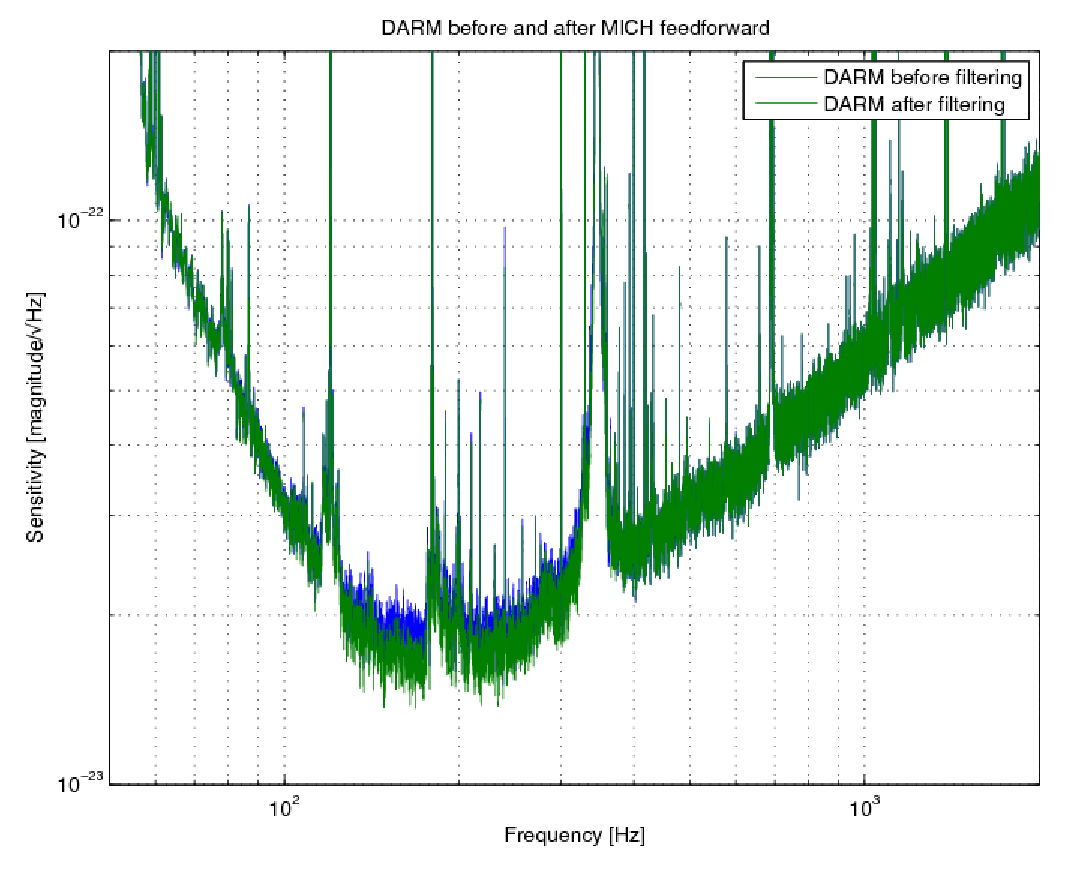
\includegraphics[height=80mm, width=60mm]{figure11.eps}
\caption{Exemplar of a typical case, +1.1 Mpc (5.9\% inspiral range)
\textit{(GPS time 953164819 to 953165839, 2010 March 21)}}
\label{typicalInspiralGraph}
\end{center}
\end{figure}
\begin{figure}
\begin{center}
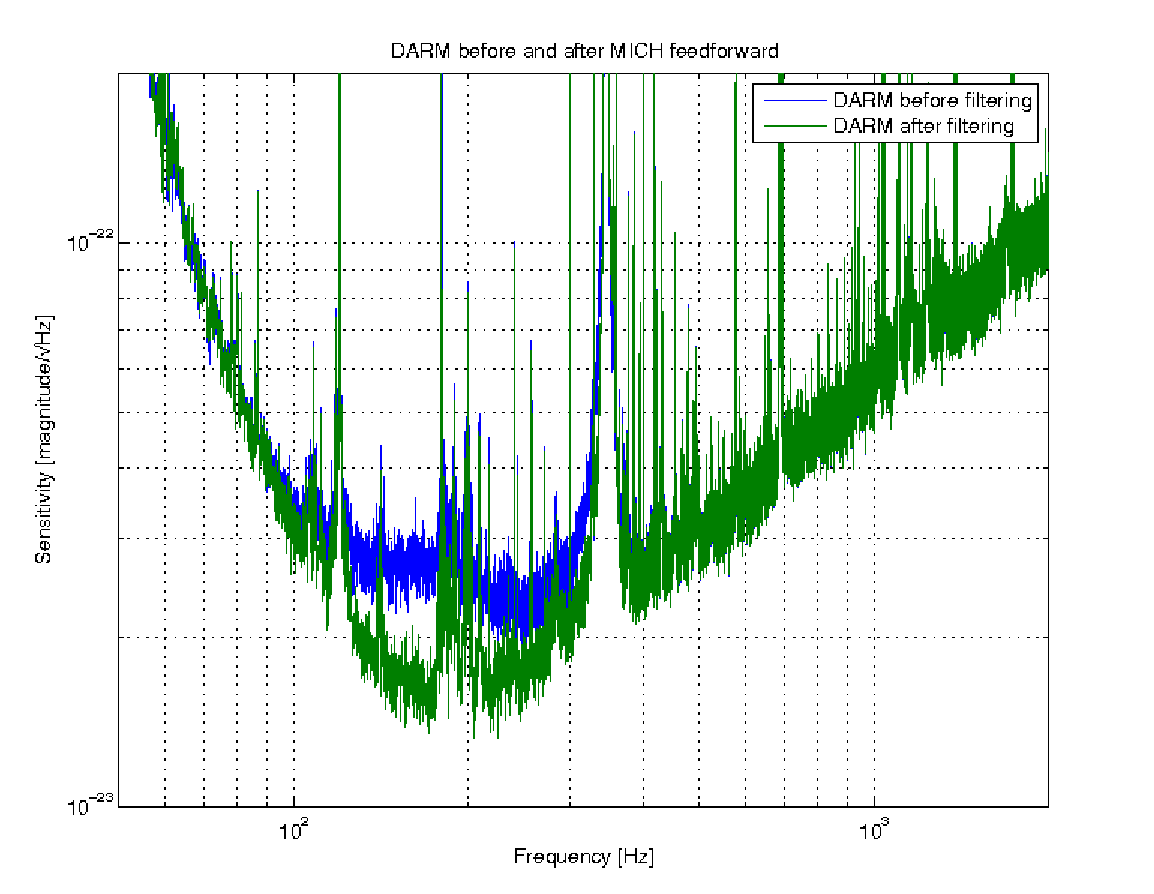
\includegraphics[height=80mm, width=60mm]{figure12.eps}
\caption{Best improvement seen in S6 for H1, +4.4 Mpc (29\% inspiral range)
\textit{(GPS 955187679 to 955188191, 2010 April 13)}}
\label{bestInspiralGraph}
\end{center}
\end{figure}

To be precise, one post-processing test computes average spectra over many windows. For this purpose, it computes Short Fourier Transforms (SFTs) of LHO data. These SFTs are short in the sense of being shorter than the duration of a (potentially year-long) science run. SFT are typically of shorter duration (typically 1800 seconds) than a science segment.  GPS seconds are measured from 1980 January 01: from GPS second $931.0\times 10^6$ (2009 July 07) to $932.8\times 10^6$ (2009 July 28, roughly the first 200 science segments of S6). We computed a harmonic mean of the spectra and compared differences and ratios, shown in Figure~\ref{SFTgraph}.

\begin{figure}
\begin{center}
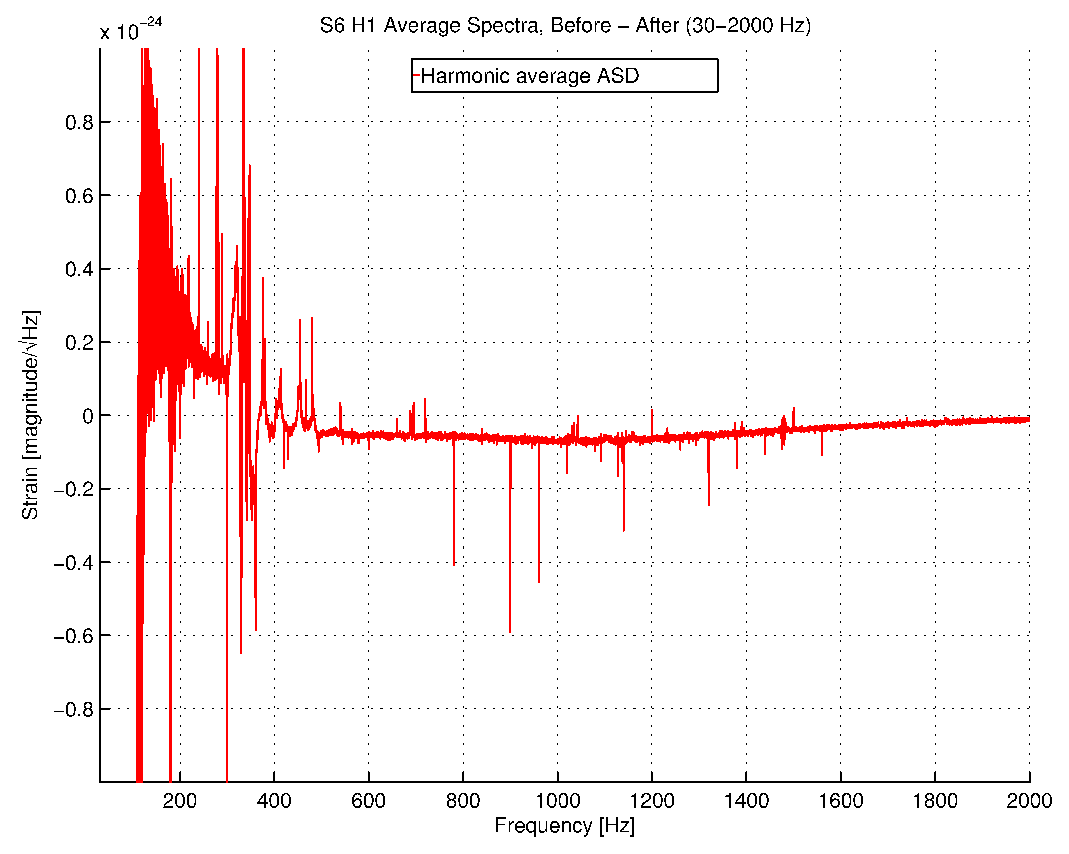
\includegraphics[height=80mm, width=60mm]{figure13a.eps}
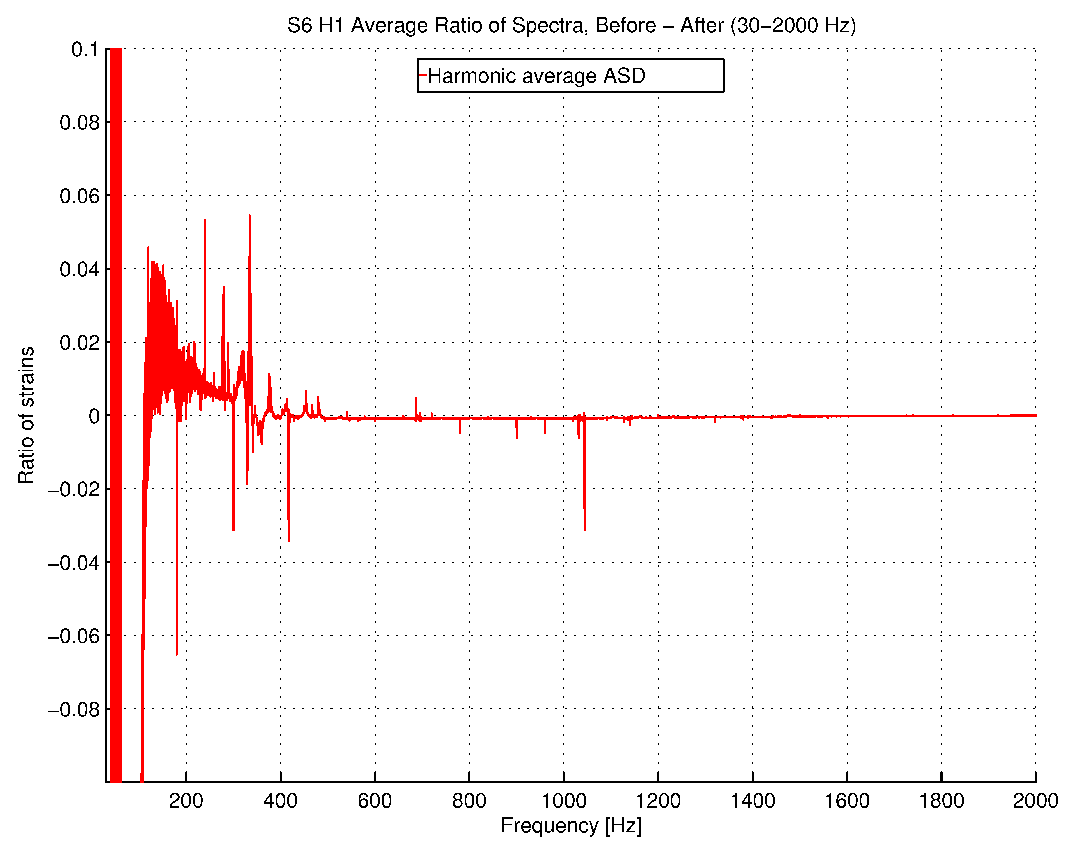
\includegraphics[height=80mm, width=60mm]{figure13b.eps}
\caption{Harmonic mean,
200 jobs from GPS second $931.0 \times 10^6$ (2009 July 07) to $932.8\times 10^6$ (2009 July 28): \textit{(before-after)} (L), \textit{(before-after)/before} (R); greater than zero is improvement.}
\label{SFTgraph}
\end{center}
\end{figure}

Note that the SFTs are high-pass filtered with a knee at 38 Hz. The harmonic mean spectrum is less susceptible to outliers than an arithmetic mean would be, and it shows a clear, several percent improvement in the band from about 80 Hz up to the violin mode frequencies. Above 400 Hz, there is slight degredation, but it is much smaller proportionally than the benefit. 

        \subsection{Feedforward benefits and potential}
        \label{benefits}

Inspiral range, the distance at which coalescing neutron stars are likely to be detected~\cite{FinnInspiral1993}, increases noticeably for both LIGO observatories when data from Science Run 6 is feedforward filtered; \textit{post facto} feedforward noise subtraction does improve performance. In future evolutions of this project, an explicit second-order correction for MICH-PRC coupling could yield marginally better performance. Real-time implementation and/or non-linear (frequency against frequency) methods might achieve more dramatic gains. Regardless, feedforward helps S6 sensitivity, and it should likewise help any observatory or science run with noise over a broad band due to residual contamination from auxiliary length control channels.

\begin{figure}
\begin{center}
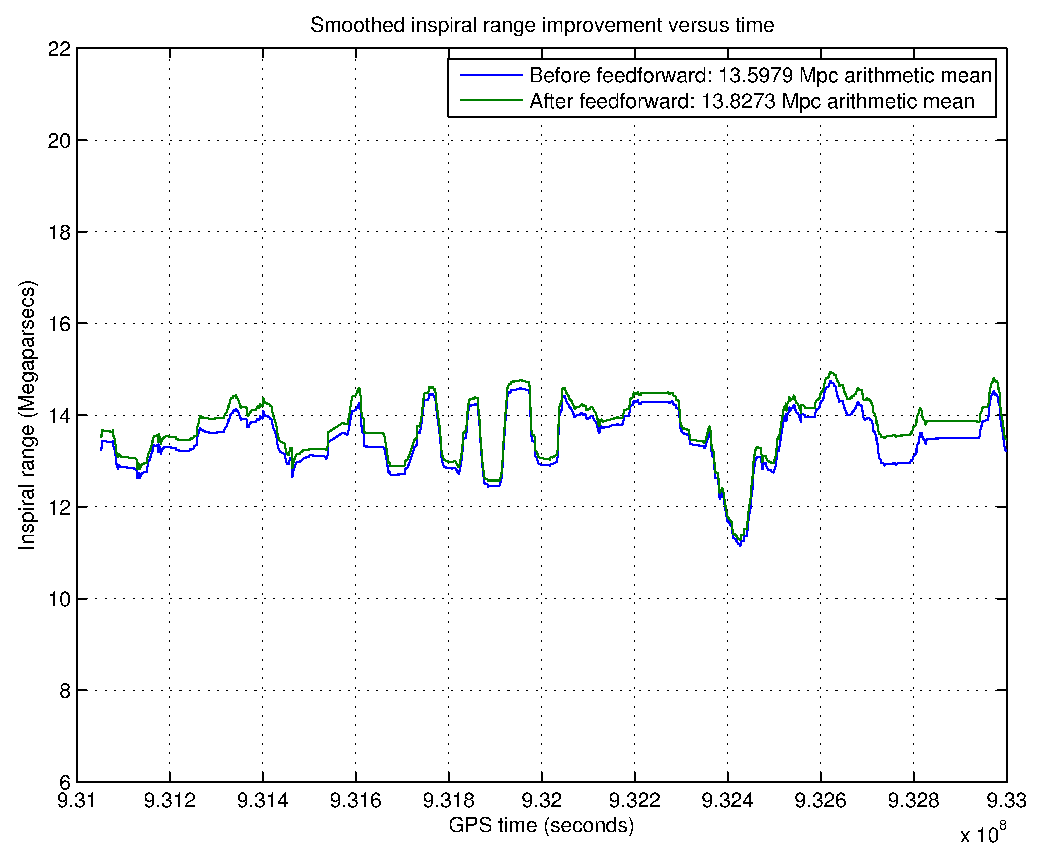
\includegraphics[height=75mm, width=150mm]{figure14a.eps}
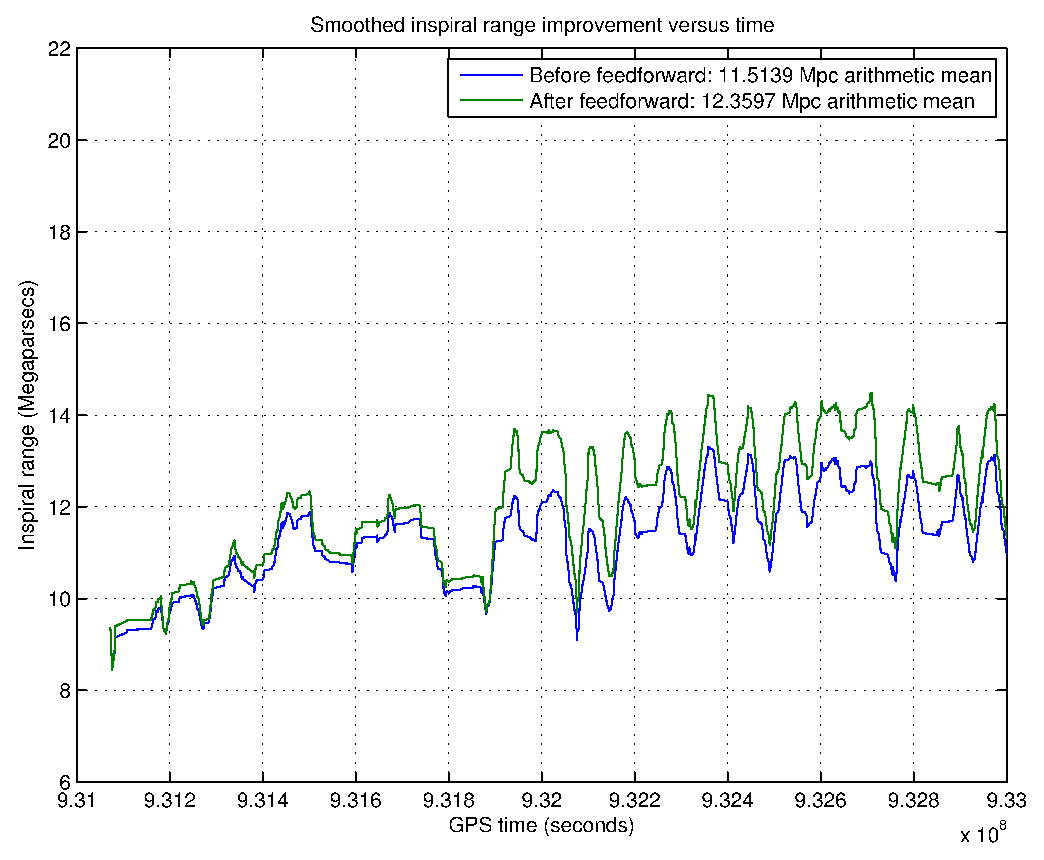
\includegraphics[height=75mm, width=150mm]{figure14b.eps}
\caption{Inspiral range vs time for Science Run 6 (starting 2009 July 07) before GPS time 9.33e8 (2009 July 30):
LIGO Hanford Observatory, H1 (top) gains 0.23 Mpc; LIGO Livingston Observatory, L1 (bottom) gains 0.84 Mpc}
\label{S6inspiralRange}
\end{center}
\end{figure}
\begin{figure}
\begin{center}
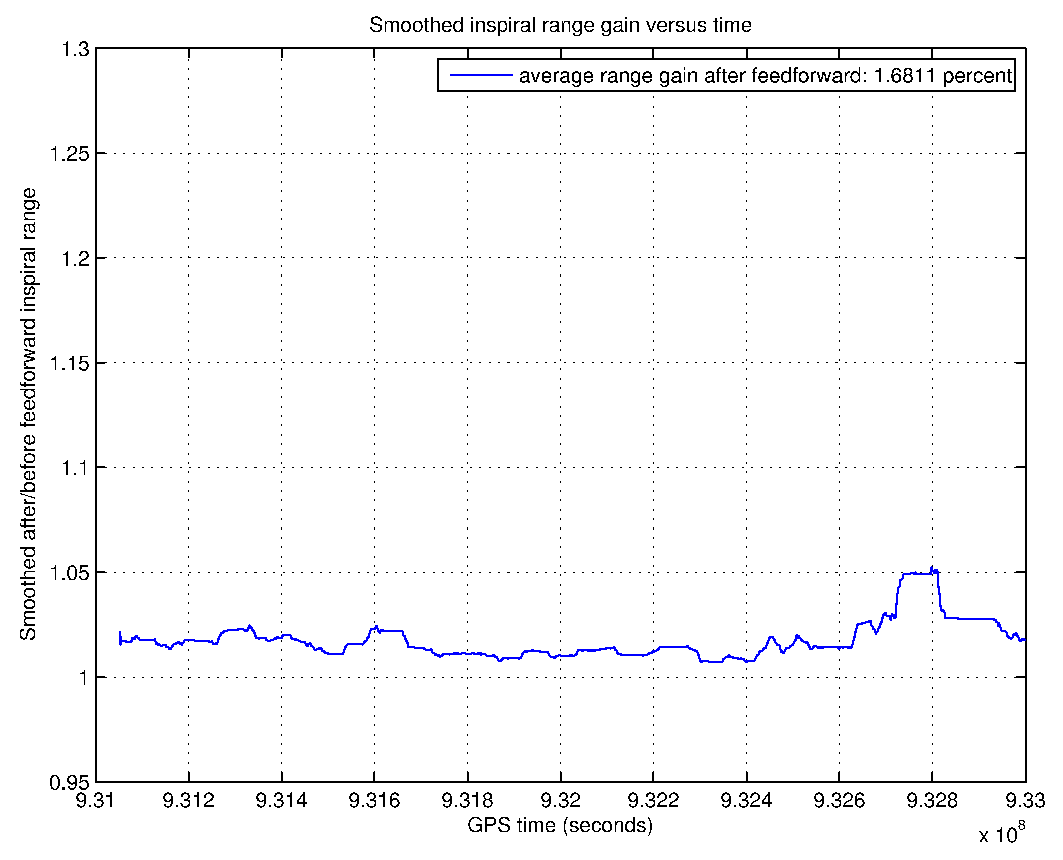
\includegraphics[height=75mm, width=150mm]{figure15a.eps}
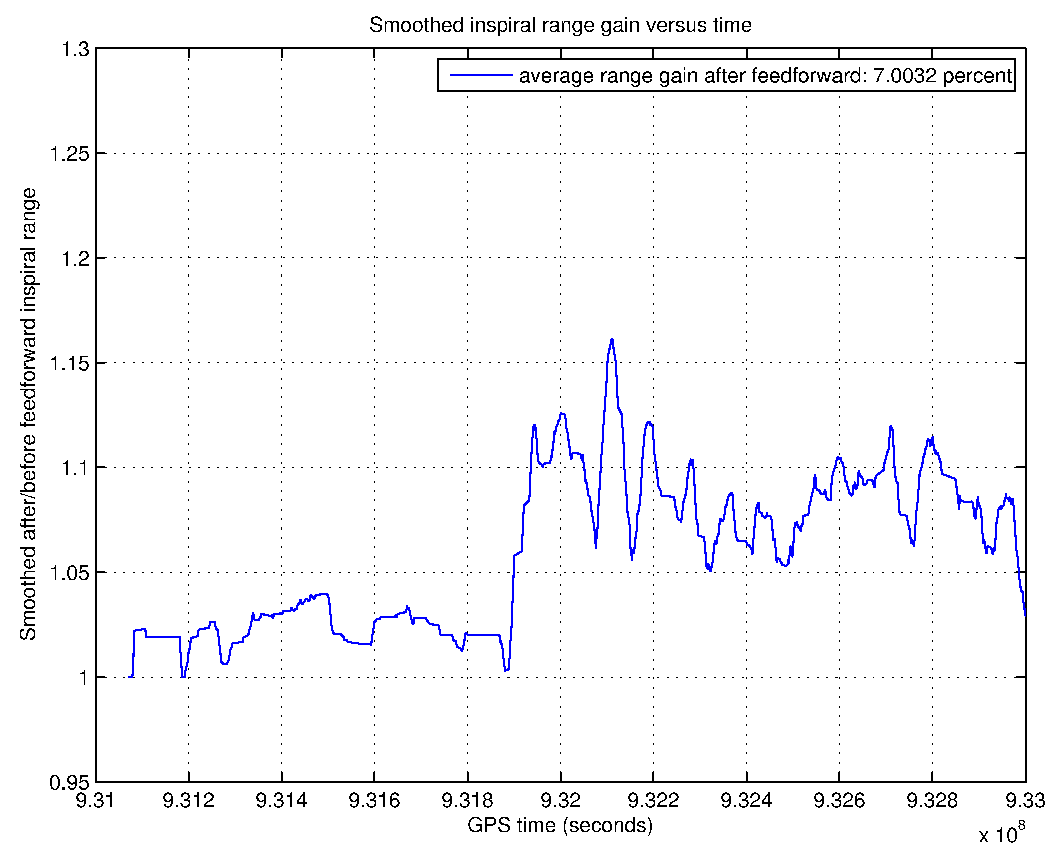
\includegraphics[height=75mm, width=150mm]{figure15b.eps}
\caption{Inspiral range \textit{fractional gain} vs time for Science Run 6 (starting 2009 July 07) before GPS time 9.33e8 (2009 July 30):
LIGO Hanford Observatory, H1 (top) 1.68\% better; LIGO Livingston Observatory, L1 (bottom) 7.00\% better}
\label{S6inspiralRangeGain}
\end{center}
\end{figure}

From Figures~\ref{S6inspiralRange} and~\ref{S6inspiralRangeGain} we can infer the variation in the MICH and PRC couplings over a 12-day sample of S6 data. Figure~\ref{diagnosticWebpages} shows a screenshot of a webpage where LIGO data analysts can access summary graphs of the feedforward performance.

\begin{figure}
\begin{center}
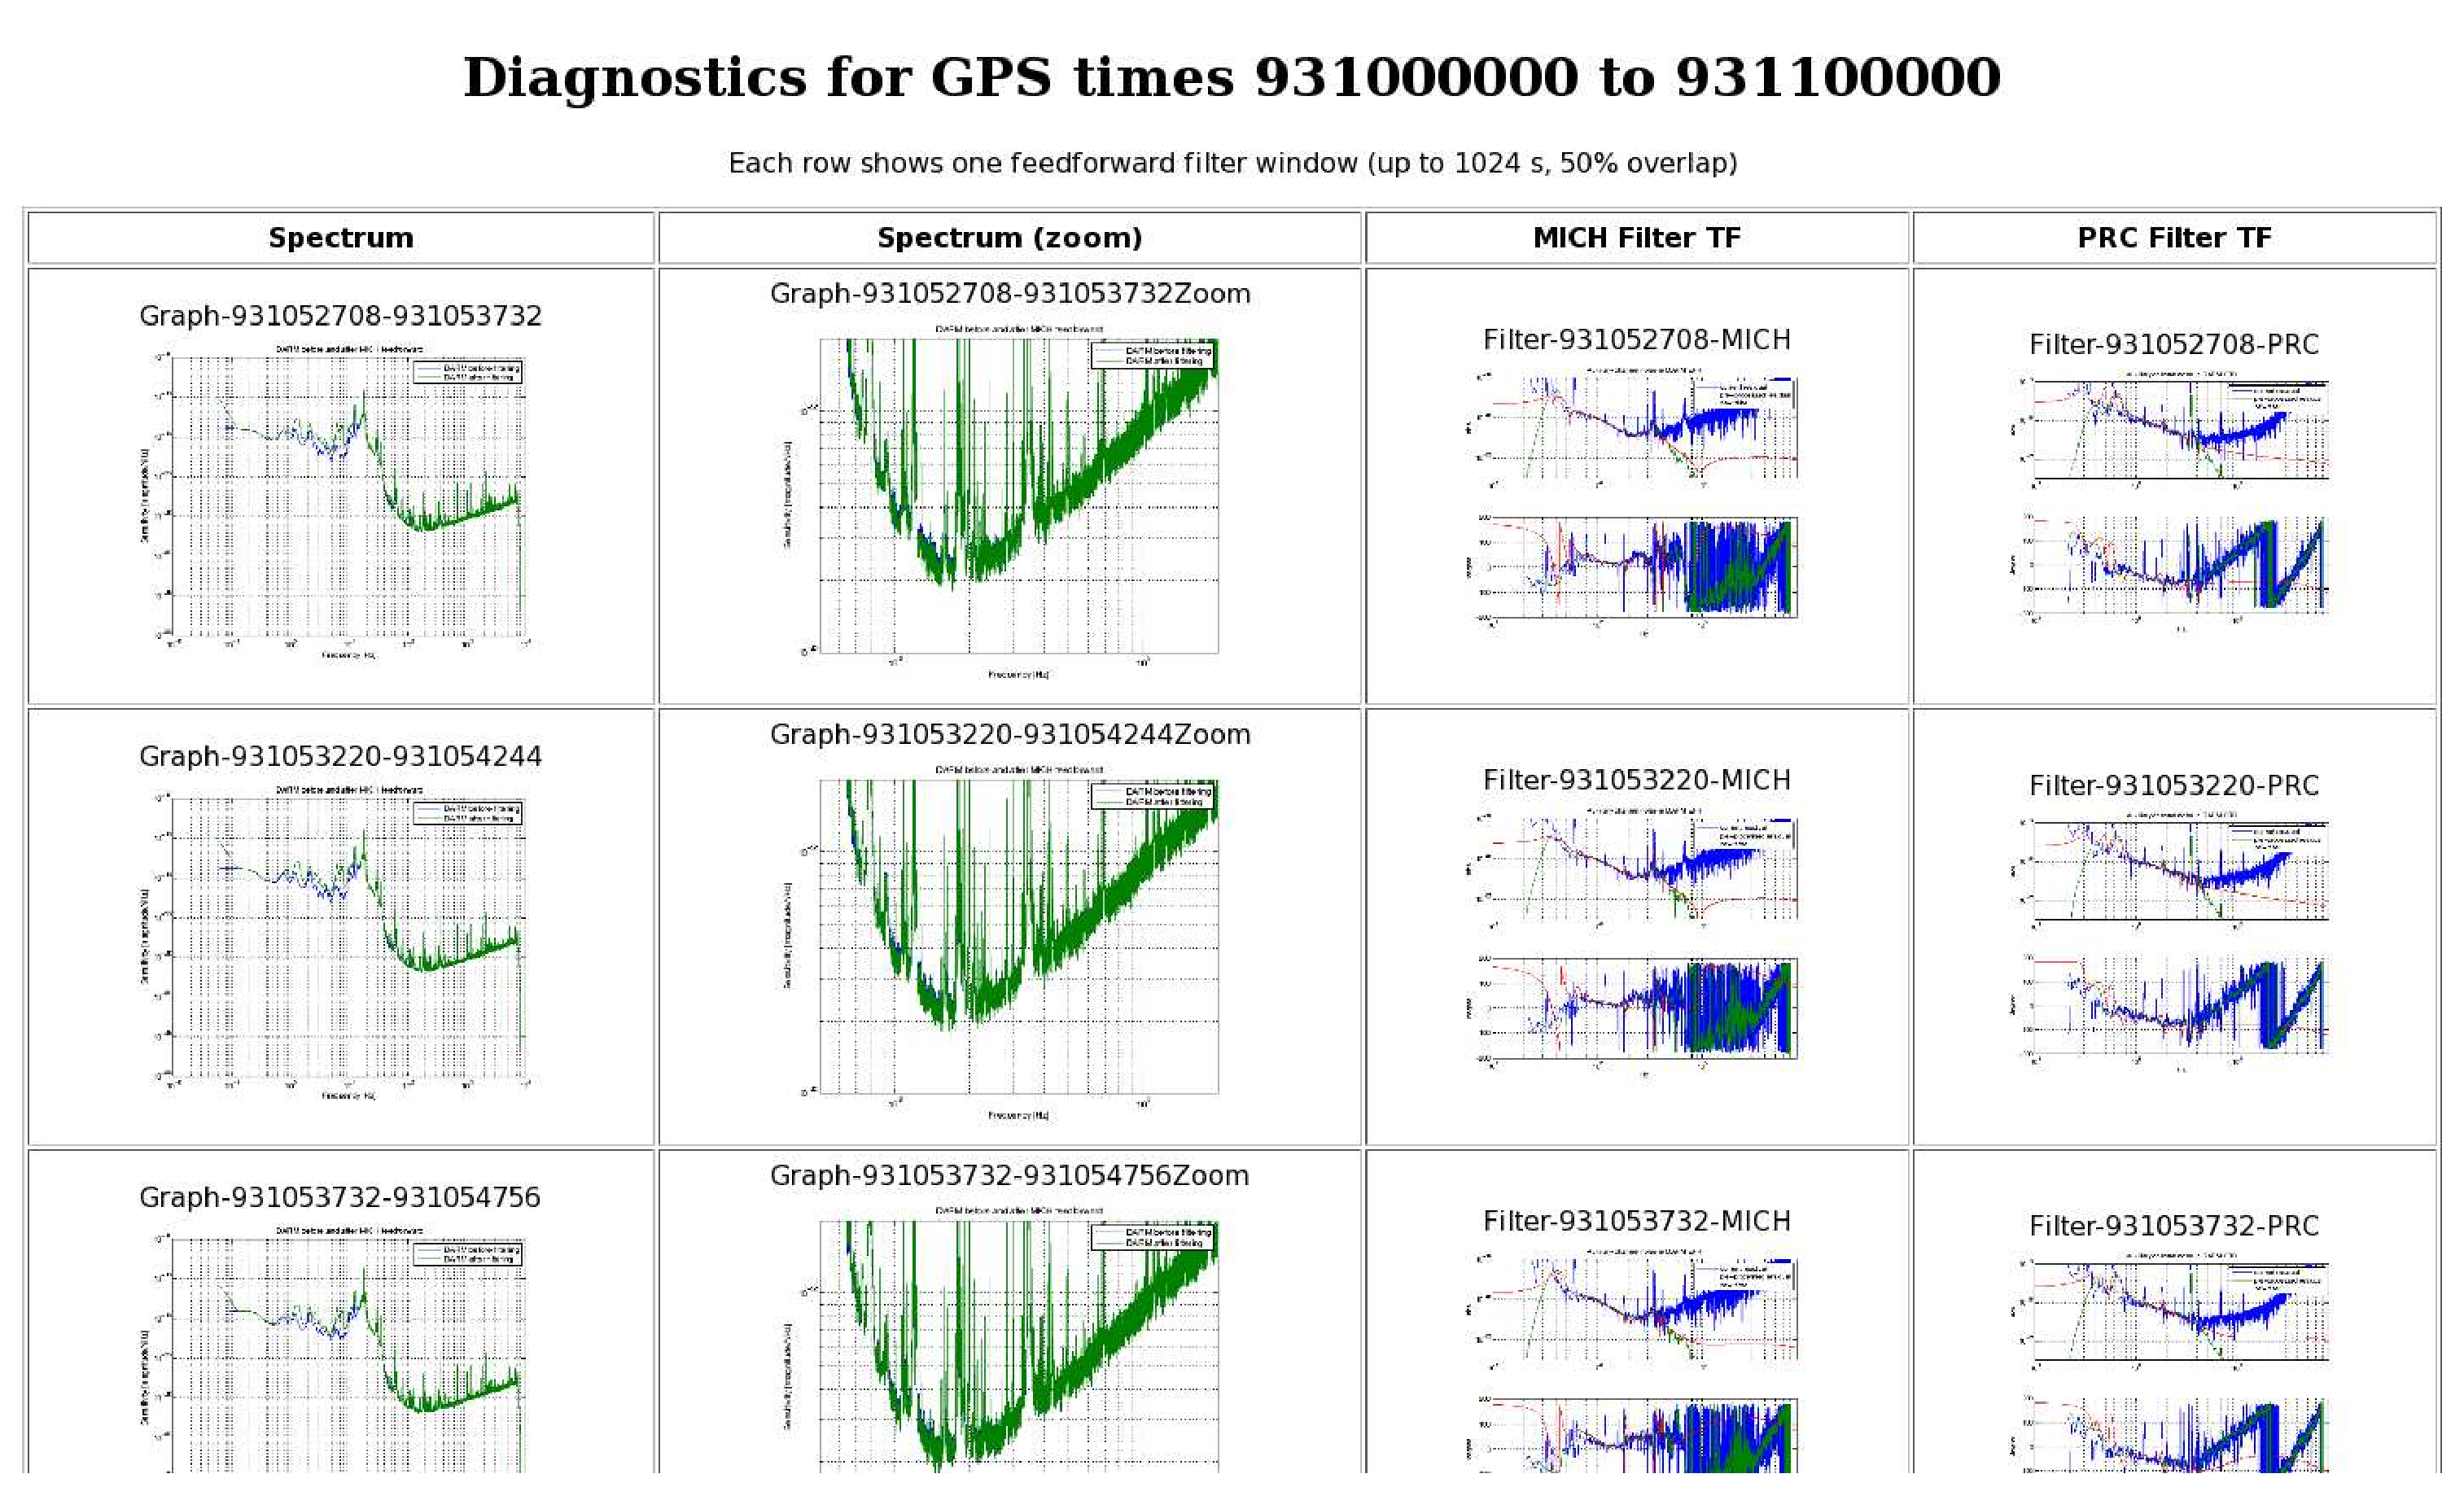
\includegraphics[height=75mm, width=150mm]{figure16.eps}
\caption{Screenshot of diagnostic web pages, indexed by window.}
\label{diagnosticWebpages}
\end{center}
\end{figure}


\section{Conclusion}

Auxiliary MICH-PRC Subtraction (AMPS) has been used to regenerate LIGO S6 data, yielding better strain sensitivity and inspiral range. Cleaned of MICH and PRC noise, data frames currently reside on the LIGO Data Grid. Frequency-domain-derived, time-domain-applied feedforward filtering removes these auxiliary length control noises by fitting a rational transfer function between noise \& signal. Second order sections filter the noise witness channels, which then sum with the measured signal to yield an improved estimate of gravitational wave strain. Matlab source code can be found at the Matapps repository~\cite{MatappsRepository}. Diagnostics confirm that $h(t)$ benefits from dynamic, adaptive, algorithmic \textit{post facto} feedforward subtraction, gaining several percent in the detectable inspiral range. This subtraction leads to the lowest noise floor in strain sensitivity around 150 Hz of any time or interferometer so far, although quantum squeezing~\cite{BarsottiNatureSqueezing,DwyerPhaseNoise} outperforms it at higher frequencies. This record may remain until Advanced LIGO begins operation. When that time comes, adaptive feedforward filters, either real-time or \textit{post facto}, can be applied to mitigate contamination from the noisy-but-inescapable parts of the tightly-coupled interferometer servo system. Signal recycling and filter cavities will only add to the complex challenge commissioning scientists face. Sensitive interferometry in years to come can benefit from simple yet effective methods of suppressing auxiliary instrumental influences.
%\end{itemize}
 
%\textit{References}:
%Note Jeff Kissel's technical report. Remember to note that Tobin Fricke wrote the function that applies the ZPKs as a SOS section-order-sections filter to the actual data, filterZPKs.m.

LIGO was constructed by the California Institute of Technology and Massachusetts Institute of Technology with funding from the National Science Foundation and operates under cooperative agreement PHY-0757058. This paper carries LIGO Document Number LIGO-P1300193. This research was also made possible by the generous support of the National Science Foundation, awards 0855422 and 1205173, LIGO Hanford Observatory, the LIGO Scientific Collaboration, and the University of Michigan. The authors wish to thank Gregory Mendell as well as Stuart Anderson, Juan Barayoga and Dan Kozak for grid computing expertise, Ian Harry for investigating signal recovery before and after injections and providing conclusions about signal-to-noise for matched filtering, Jeff Kissel for refining MICH and PRC subtraction by hand, Tobin Fricke for the filtering function, and Rana Adhikari and Jenne Driggers for developing many of these methods at the Caltech 40 m interferometer.

%\appendix


%\section*{References}
%\bibliographystyle{jphysicsB}
%\bibliography{Meadors_LIGO_AMPS_feedforward}
%\begin{thebibliography}
%\bibitem{book1} Goosens M, Rahtz S and Mittelbach F 1997 {\it The \LaTeX\ Graphics Companion\/} 
%(Reading, MA: Addison-Wesley)
%\bibitem{eps} Reckdahl K 1997 {\it Using Imported Graphics in \LaTeX\ } (search 
%CTAN for the file `epslatex.pdf')
%\References
%\bibitem{AdhikariThesis} Adhikari R
%\bibitem{AllenHuaOttawill1999}
%\bibitem{BallmerThesis}
%\bibitem{Deschrijver2008}
%\bibitem{Gustavsen1999}
%\bibitem{Gustavsen2006}
%\bibitem{KissellPRCMICH} Kissel J {\it MICH and PRC coupling into DARM} (web: \verbatim{http://ilog.ligo-wa.caltech.edu/ilog/pub/ilog.cgi?group=detector\& date\_to\_view=06/16/2009\&anchor\_to\_scroll\_to=2009:06:16:23:51:59-kissel})
%\endrefs
%\end{thebibliography}

%\end{document}

